\documentclass[1p]{elsarticle_modified}
%\bibliographystyle{elsarticle-num}

%\usepackage[colorlinks]{hyperref}
%\usepackage{abbrmath_seonhwa} %\Abb, \Ascr, \Acal ,\Abf, \Afrak
\usepackage{amsfonts}
\usepackage{amssymb}
\usepackage{amsmath}
\usepackage{amsthm}
\usepackage{scalefnt}
\usepackage{amsbsy}
\usepackage{kotex}
\usepackage{caption}
\usepackage{subfig}
\usepackage{color}
\usepackage{graphicx}
\usepackage{xcolor} %% white, black, red, green, blue, cyan, magenta, yellow
\usepackage{float}
\usepackage{setspace}
\usepackage{hyperref}

\usepackage{tikz}
\usetikzlibrary{arrows}

\usepackage{multirow}
\usepackage{array} % fixed length table
\usepackage{hhline}

%%%%%%%%%%%%%%%%%%%%%
\makeatletter
\renewcommand*\env@matrix[1][\arraystretch]{%
	\edef\arraystretch{#1}%
	\hskip -\arraycolsep
	\let\@ifnextchar\new@ifnextchar
	\array{*\c@MaxMatrixCols c}}
\makeatother %https://tex.stackexchange.com/questions/14071/how-can-i-increase-the-line-spacing-in-a-matrix
%%%%%%%%%%%%%%%

\usepackage[normalem]{ulem}

\newcommand{\msout}[1]{\ifmmode\text{\sout{\ensuremath{#1}}}\else\sout{#1}\fi}
%SOURCE: \msout is \stkout macro in https://tex.stackexchange.com/questions/20609/strikeout-in-math-mode

\newcommand{\cancel}[1]{
	\ifmmode
	{\color{red}\msout{#1}}
	\else
	{\color{red}\sout{#1}}
	\fi
}

\newcommand{\add}[1]{
	{\color{blue}\uwave{#1}}
}

\newcommand{\replace}[2]{
	\ifmmode
	{\color{red}\msout{#1}}{\color{blue}\uwave{#2}}
	\else
	{\color{red}\sout{#1}}{\color{blue}\uwave{#2}}
	\fi
}

\newcommand{\Sol}{\mathcal{S}} %segment
\newcommand{\D}{D} %diagram
\newcommand{\A}{\mathcal{A}} %arc


%%%%%%%%%%%%%%%%%%%%%%%%%%%%%5 test

\def\sl{\operatorname{\textup{SL}}(2,\Cbb)}
\def\psl{\operatorname{\textup{PSL}}(2,\Cbb)}
\def\quan{\mkern 1mu \triangleright \mkern 1mu}

\theoremstyle{definition}
\newtheorem{thm}{Theorem}[section]
\newtheorem{prop}[thm]{Proposition}
\newtheorem{lem}[thm]{Lemma}
\newtheorem{ques}[thm]{Question}
\newtheorem{cor}[thm]{Corollary}
\newtheorem{defn}[thm]{Definition}
\newtheorem{exam}[thm]{Example}
\newtheorem{rmk}[thm]{Remark}
\newtheorem{alg}[thm]{Algorithm}

\newcommand{\I}{\sqrt{-1}}
\begin{document}

%\begin{frontmatter}
%
%\title{Boundary parabolic representations of knots up to 8 crossings}
%
%%% Group authors per affiliation:
%\author{Yunhi Cho} 
%\address{Department of Mathematics, University of Seoul, Seoul, Korea}
%\ead{yhcho@uos.ac.kr}
%
%
%\author{Seonhwa Kim} %\fnref{s_kim}}
%\address{Center for Geometry and Physics, Institute for Basic Science, Pohang, 37673, Korea}
%\ead{ryeona17@ibs.re.kr}
%
%\author{Hyuk Kim}
%\address{Department of Mathematical Sciences, Seoul National University, Seoul 08826, Korea}
%\ead{hyukkim@snu.ac.kr}
%
%\author{Seokbeom Yoon}
%\address{Department of Mathematical Sciences, Seoul National University, Seoul, 08826,  Korea}
%\ead{sbyoon15@snu.ac.kr}
%
%\begin{abstract}
%We find all boundary parabolic representation of knots up to 8 crossings.
%
%\end{abstract}
%\begin{keyword}
%    \MSC[2010] 57M25 
%\end{keyword}
%
%\end{frontmatter}

%\linenumbers
%\tableofcontents
%
\newcommand\colored[1]{\textcolor{white}{\rule[-0.35ex]{0.8em}{1.4ex}}\kern-0.8em\color{red} #1}%
%\newcommand\colored[1]{\textcolor{white}{ #1}\kern-2.17ex	\textcolor{white}{ #1}\kern-1.81ex	\textcolor{white}{ #1}\kern-2.15ex\color{red}#1	}

{\Large $\underline{12a_{0407}~(K12a_{0407})}$}

\setlength{\tabcolsep}{10pt}
\renewcommand{\arraystretch}{1.6}
\vspace{1cm}\begin{tabular}{m{100pt}>{\centering\arraybackslash}m{274pt}}
\multirow{5}{120pt}{
	\centering
	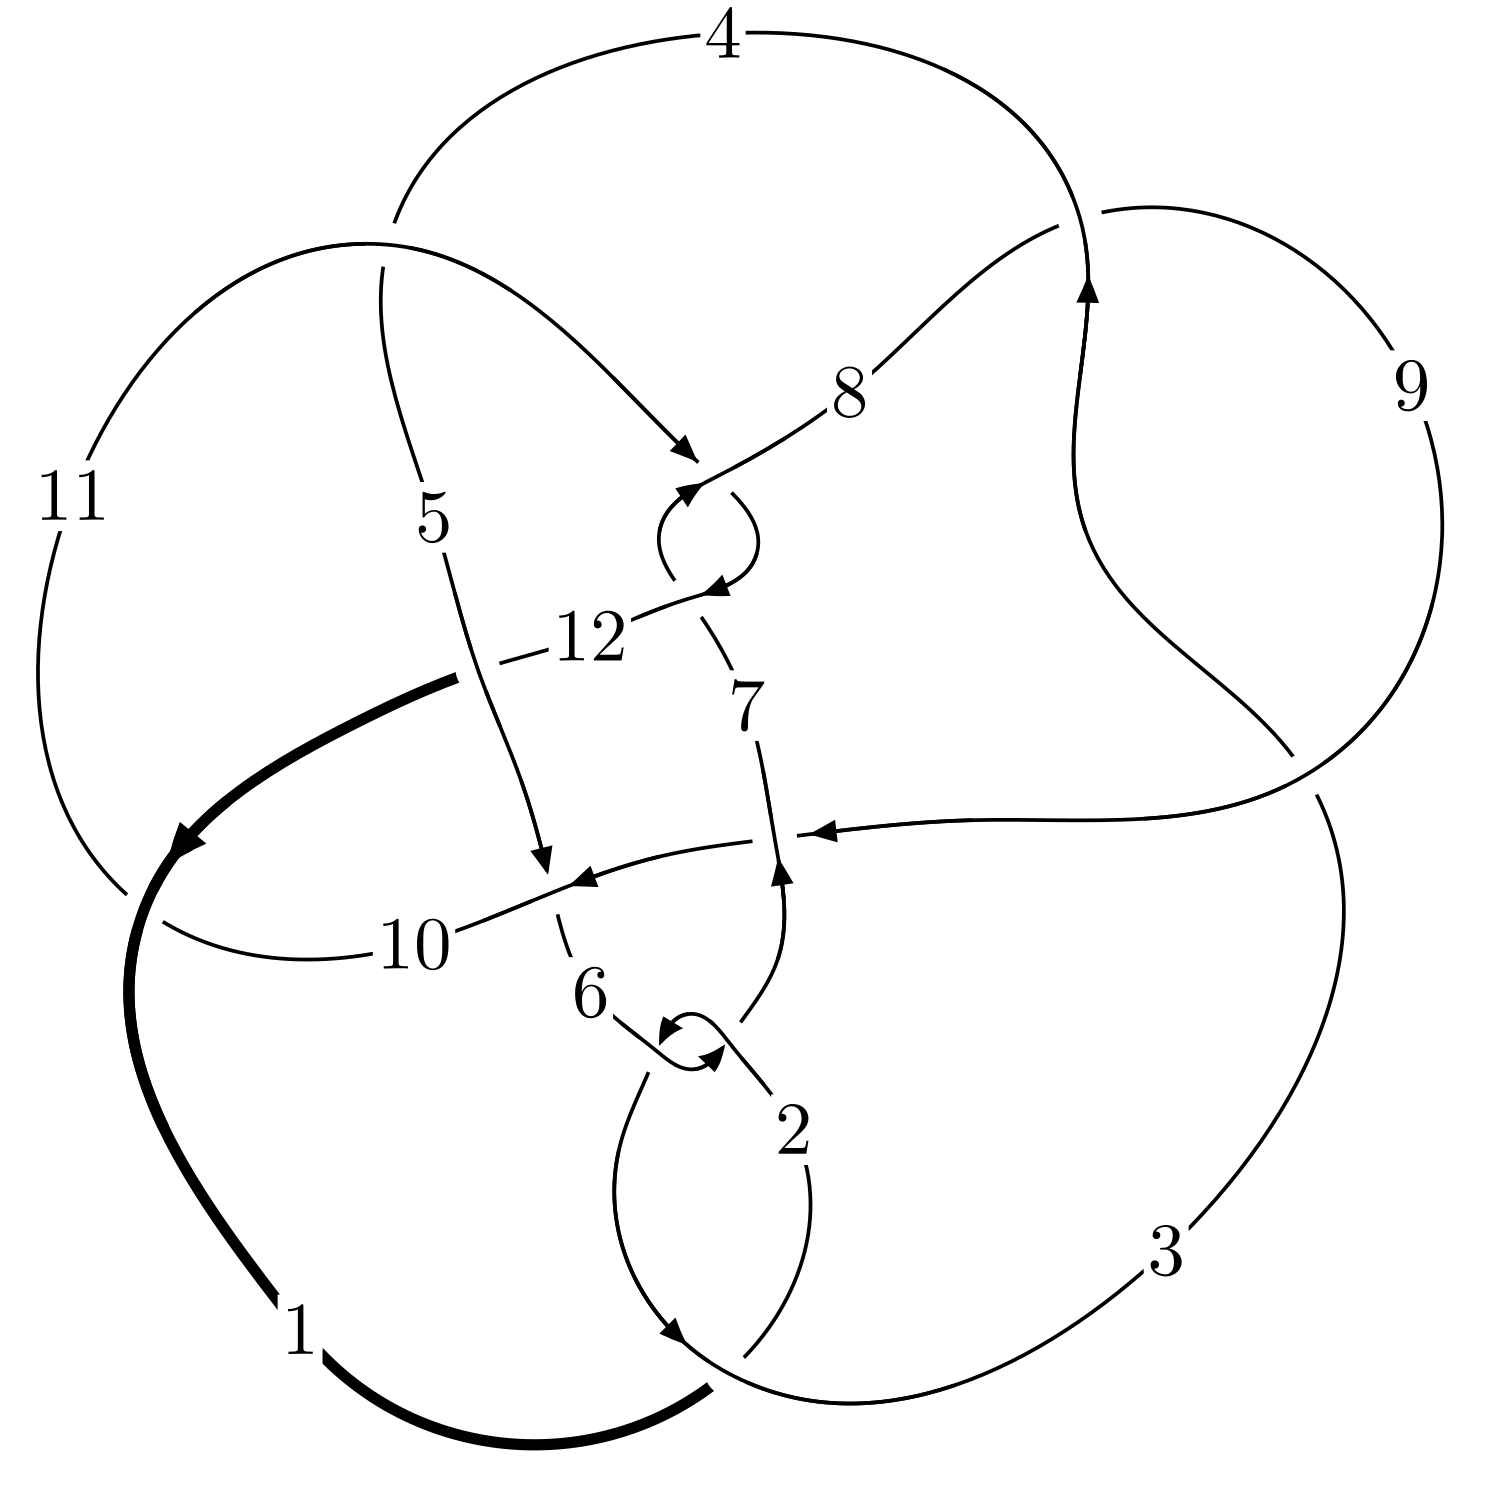
\includegraphics[width=112pt]{../../../GIT/diagram.site/Diagrams/png/1208_12a_0407.png}\\
\ \ \ A knot diagram\footnotemark}&
\allowdisplaybreaks
\textbf{Linearized knot diagam} \\
\cline{2-2}
 &
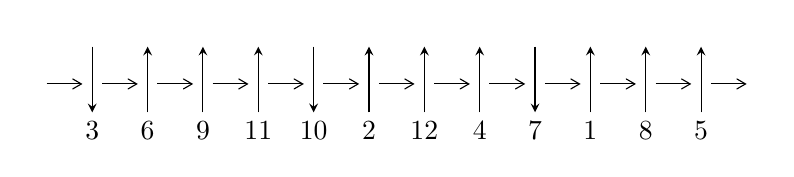
\begin{tikzpicture}[x=20pt, y=17pt]
	% nodes
	\node (C0) at (0, 0) {};
	\node (C1) at (1, 0) {};
	\node (C1U) at (1, +1) {};
	\node (C1D) at (1, -1) {3};

	\node (C2) at (2, 0) {};
	\node (C2U) at (2, +1) {};
	\node (C2D) at (2, -1) {6};

	\node (C3) at (3, 0) {};
	\node (C3U) at (3, +1) {};
	\node (C3D) at (3, -1) {9};

	\node (C4) at (4, 0) {};
	\node (C4U) at (4, +1) {};
	\node (C4D) at (4, -1) {11};

	\node (C5) at (5, 0) {};
	\node (C5U) at (5, +1) {};
	\node (C5D) at (5, -1) {10};

	\node (C6) at (6, 0) {};
	\node (C6U) at (6, +1) {};
	\node (C6D) at (6, -1) {2};

	\node (C7) at (7, 0) {};
	\node (C7U) at (7, +1) {};
	\node (C7D) at (7, -1) {12};

	\node (C8) at (8, 0) {};
	\node (C8U) at (8, +1) {};
	\node (C8D) at (8, -1) {4};

	\node (C9) at (9, 0) {};
	\node (C9U) at (9, +1) {};
	\node (C9D) at (9, -1) {7};

	\node (C10) at (10, 0) {};
	\node (C10U) at (10, +1) {};
	\node (C10D) at (10, -1) {1};

	\node (C11) at (11, 0) {};
	\node (C11U) at (11, +1) {};
	\node (C11D) at (11, -1) {8};

	\node (C12) at (12, 0) {};
	\node (C12U) at (12, +1) {};
	\node (C12D) at (12, -1) {5};
	\node (C13) at (13, 0) {};

	% arrows
	\draw[->,>={angle 60}]
	(C0) edge (C1) (C1) edge (C2) (C2) edge (C3) (C3) edge (C4) (C4) edge (C5) (C5) edge (C6) (C6) edge (C7) (C7) edge (C8) (C8) edge (C9) (C9) edge (C10) (C10) edge (C11) (C11) edge (C12) (C12) edge (C13) ;	\draw[->,>=stealth]
	(C1U) edge (C1D) (C2D) edge (C2U) (C3D) edge (C3U) (C4D) edge (C4U) (C5U) edge (C5D) (C6D) edge (C6U) (C7D) edge (C7U) (C8D) edge (C8U) (C9U) edge (C9D) (C10D) edge (C10U) (C11D) edge (C11U) (C12D) edge (C12U) ;
	\end{tikzpicture} \\
\hhline{~~} \\& 
\textbf{Solving Sequence} \\ \cline{2-2} 
 &
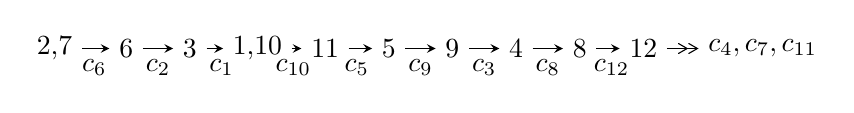
\begin{tikzpicture}[x=23pt, y=7pt]
	% node
	\node (A0) at (-1/8, 0) {2,7};
	\node (A1) at (1, 0) {6};
	\node (A2) at (2, 0) {3};
	\node (A3) at (49/16, 0) {1,10};
	\node (A4) at (33/8, 0) {11};
	\node (A5) at (41/8, 0) {5};
	\node (A6) at (49/8, 0) {9};
	\node (A7) at (57/8, 0) {4};
	\node (A8) at (65/8, 0) {8};
	\node (A9) at (73/8, 0) {12};
	\node (C1) at (1/2, -1) {$c_{6}$};
	\node (C2) at (3/2, -1) {$c_{2}$};
	\node (C3) at (5/2, -1) {$c_{1}$};
	\node (C4) at (29/8, -1) {$c_{10}$};
	\node (C5) at (37/8, -1) {$c_{5}$};
	\node (C6) at (45/8, -1) {$c_{9}$};
	\node (C7) at (53/8, -1) {$c_{3}$};
	\node (C8) at (61/8, -1) {$c_{8}$};
	\node (C9) at (69/8, -1) {$c_{12}$};
	\node (A10) at (11, 0) {$c_{4},c_{7},c_{11}$};

	% edge
	\draw[->,>=stealth]	
	(A0) edge (A1) (A1) edge (A2) (A2) edge (A3) (A3) edge (A4) (A4) edge (A5) (A5) edge (A6) (A6) edge (A7) (A7) edge (A8) (A8) edge (A9) ;
	\draw[->>,>={angle 60}]	
	(A9) edge (A10);
\end{tikzpicture} \\ 

\end{tabular} \\

\footnotetext{
The image of knot diagram is generated by the software ``\textbf{Draw programme}" developed by Andrew Bartholomew(\url{http://www.layer8.co.uk/maths/draw/index.htm\#Running-draw}), where we modified some parts for our purpose(\url{https://github.com/CATsTAILs/LinksPainter}).
}\phantom \\ \newline 
\centering \textbf{Ideals for irreducible components\footnotemark of $X_{\text{par}}$} 
 
\begin{align*}
I^u_{1}&=\langle 
7.29009\times10^{364} u^{160}+5.02475\times10^{364} u^{159}+\cdots+1.34269\times10^{365} b+1.27656\times10^{366},\\
\phantom{I^u_{1}}&\phantom{= \langle  }1.16613\times10^{365} u^{160}+5.58206\times10^{365} u^{159}+\cdots+1.34269\times10^{365} a+3.05746\times10^{366},\;u^{161}+u^{160}+\cdots-17 u-1\rangle \\
I^u_{2}&=\langle 
-273942 u^{35}+8823771 u^{34}+\cdots+3079049 b+13356427,\\
\phantom{I^u_{2}}&\phantom{= \langle  }24459491 u^{35}+69731434 u^{34}+\cdots+9237147 a+438577488,\;u^{36}+2 u^{35}+\cdots+22 u^2+3\rangle \\
\\
\end{align*}
\raggedright * 2 irreducible components of $\dim_{\mathbb{C}}=0$, with total 197 representations.\\
\footnotetext{All coefficients of polynomials are rational numbers. But the coefficients are sometimes approximated in decimal forms when there is not enough margin.}
\newpage
\renewcommand{\arraystretch}{1}
\centering \section*{I. $I^u_{1}= \langle 7.29\times10^{364} u^{160}+5.02\times10^{364} u^{159}+\cdots+1.34\times10^{365} b+1.28\times10^{366},\;1.17\times10^{365} u^{160}+5.58\times10^{365} u^{159}+\cdots+1.34\times10^{365} a+3.06\times10^{366},\;u^{161}+u^{160}+\cdots-17 u-1 \rangle$}
\flushleft \textbf{(i) Arc colorings}\\
\begin{tabular}{m{7pt} m{180pt} m{7pt} m{180pt} }
\flushright $a_{2}=$&$\begin{pmatrix}0\\u\end{pmatrix}$ \\
\flushright $a_{7}=$&$\begin{pmatrix}1\\0\end{pmatrix}$ \\
\flushright $a_{6}=$&$\begin{pmatrix}1\\u^2\end{pmatrix}$ \\
\flushright $a_{3}=$&$\begin{pmatrix}u\\u^3+u\end{pmatrix}$ \\
\flushright $a_{1}=$&$\begin{pmatrix}u^3\\u^5+u^3+u\end{pmatrix}$ \\
\flushright $a_{10}=$&$\begin{pmatrix}-0.868503 u^{160}-4.15736 u^{159}+\cdots-244.015 u-22.7711\\-0.542945 u^{160}-0.374229 u^{159}+\cdots-120.551 u-9.50743\end{pmatrix}$ \\
\flushright $a_{11}=$&$\begin{pmatrix}-6.83002 u^{160}-10.0892 u^{159}+\cdots-334.168 u-28.0262\\0.493273 u^{160}+3.42162 u^{159}+\cdots-154.528 u-11.2426\end{pmatrix}$ \\
\flushright $a_{5}=$&$\begin{pmatrix}-3.32957 u^{160}-11.0086 u^{159}+\cdots+264.354 u+24.6671\\0.172703 u^{160}+0.694748 u^{159}+\cdots+58.0416 u+7.08239\end{pmatrix}$ \\
\flushright $a_{9}=$&$\begin{pmatrix}-1.41145 u^{160}-4.53159 u^{159}+\cdots-364.565 u-32.2785\\-0.542945 u^{160}-0.374229 u^{159}+\cdots-120.551 u-9.50743\end{pmatrix}$ \\
\flushright $a_{4}=$&$\begin{pmatrix}1.59253 u^{160}+1.09474 u^{159}+\cdots+68.7446 u+6.82380\\6.15262 u^{160}+11.1489 u^{159}+\cdots+25.3152 u+2.66973\end{pmatrix}$ \\
\flushright $a_{8}=$&$\begin{pmatrix}49.0445 u^{160}+47.6382 u^{159}+\cdots+457.132 u+19.3973\\2.26467 u^{160}+2.11722 u^{159}+\cdots-30.9504 u-4.04200\end{pmatrix}$ \\
\flushright $a_{12}=$&$\begin{pmatrix}-73.2349 u^{160}-125.571 u^{159}+\cdots-55.2086 u+1.05695\\0.935533 u^{160}+3.82850 u^{159}+\cdots+24.5975 u+4.26703\end{pmatrix}$\\&\end{tabular}
\flushleft \textbf{(ii) Obstruction class $= -1$}\\~\\
\flushleft \textbf{(iii) Cusp Shapes $= 69.0866 u^{160}+87.1460 u^{159}+\cdots+242.322 u+5.30831$}\\~\\
\newpage\renewcommand{\arraystretch}{1}
\flushleft \textbf{(iv) u-Polynomials at the component}\newline \\
\begin{tabular}{m{50pt}|m{274pt}}
Crossings & \hspace{64pt}u-Polynomials at each crossing \\
\hline $$\begin{aligned}c_{1}\end{aligned}$$&$\begin{aligned}
&u^{161}+77 u^{160}+\cdots+87 u-1
\end{aligned}$\\
\hline $$\begin{aligned}c_{2},c_{6}\end{aligned}$$&$\begin{aligned}
&u^{161}+u^{160}+\cdots-17 u-1
\end{aligned}$\\
\hline $$\begin{aligned}c_{3},c_{8}\end{aligned}$$&$\begin{aligned}
&u^{161}-3 u^{160}+\cdots+4109148 u-232661
\end{aligned}$\\
\hline $$\begin{aligned}c_{4}\end{aligned}$$&$\begin{aligned}
&u^{161}+31 u^{159}+\cdots-835953597 u-981193891
\end{aligned}$\\
\hline $$\begin{aligned}c_{5}\end{aligned}$$&$\begin{aligned}
&u^{161}-2 u^{160}+\cdots+54544 u-4861
\end{aligned}$\\
\hline $$\begin{aligned}c_{7},c_{11}\end{aligned}$$&$\begin{aligned}
&u^{161}+u^{160}+\cdots-57047 u-4381
\end{aligned}$\\
\hline $$\begin{aligned}c_{9}\end{aligned}$$&$\begin{aligned}
&u^{161}-16 u^{160}+\cdots+9283 u-167
\end{aligned}$\\
\hline $$\begin{aligned}c_{10}\end{aligned}$$&$\begin{aligned}
&u^{161}+17 u^{160}+\cdots-158166 u-7087
\end{aligned}$\\
\hline $$\begin{aligned}c_{12}\end{aligned}$$&$\begin{aligned}
&u^{161}- u^{160}+\cdots-31 u-1
\end{aligned}$\\
\hline
\end{tabular}\\~\\
\newpage\renewcommand{\arraystretch}{1}
\flushleft \textbf{(v) Riley Polynomials at the component}\newline \\
\begin{tabular}{m{50pt}|m{274pt}}
Crossings & \hspace{64pt}Riley Polynomials at each crossing \\
\hline $$\begin{aligned}c_{1}\end{aligned}$$&$\begin{aligned}
&y^{161}+29 y^{160}+\cdots+4223 y-1
\end{aligned}$\\
\hline $$\begin{aligned}c_{2},c_{6}\end{aligned}$$&$\begin{aligned}
&y^{161}+77 y^{160}+\cdots+87 y-1
\end{aligned}$\\
\hline $$\begin{aligned}c_{3},c_{8}\end{aligned}$$&$\begin{aligned}
&y^{161}+123 y^{160}+\cdots+6872989493074 y-54131140921
\end{aligned}$\\
\hline $$\begin{aligned}c_{4}\end{aligned}$$&$\begin{aligned}
&y^{161}+62 y^{160}+\cdots-1.81\times10^{19} y-9.63\times10^{17}
\end{aligned}$\\
\hline $$\begin{aligned}c_{5}\end{aligned}$$&$\begin{aligned}
&y^{161}+14 y^{160}+\cdots+3371540262 y-23629321
\end{aligned}$\\
\hline $$\begin{aligned}c_{7},c_{11}\end{aligned}$$&$\begin{aligned}
&y^{161}+107 y^{160}+\cdots-1600208367 y-19193161
\end{aligned}$\\
\hline $$\begin{aligned}c_{9}\end{aligned}$$&$\begin{aligned}
&y^{161}-18 y^{160}+\cdots+18773891 y-27889
\end{aligned}$\\
\hline $$\begin{aligned}c_{10}\end{aligned}$$&$\begin{aligned}
&y^{161}-5 y^{160}+\cdots-2043156540 y-50225569
\end{aligned}$\\
\hline $$\begin{aligned}c_{12}\end{aligned}$$&$\begin{aligned}
&y^{161}+9 y^{160}+\cdots-771 y-1
\end{aligned}$\\
\hline
\end{tabular}\\~\\
\newpage\flushleft \textbf{(vi) Complex Volumes and Cusp Shapes}
$$\begin{array}{c|c|c}  
\text{Solutions to }I^u_{1}& \I (\text{vol} + \sqrt{-1}CS) & \text{Cusp shape}\\
 \hline 
\begin{aligned}
u &= \phantom{-}0.920183 + 0.388318 I \\
a &= -0.120462 + 0.084381 I \\
b &= -1.05456 - 1.26768 I\end{aligned}
 & -4.4461 - 14.5339 I & \phantom{-0.000000 } 0 \\ \hline\begin{aligned}
u &= \phantom{-}0.920183 - 0.388318 I \\
a &= -0.120462 - 0.084381 I \\
b &= -1.05456 + 1.26768 I\end{aligned}
 & -4.4461 + 14.5339 I & \phantom{-0.000000 } 0 \\ \hline\begin{aligned}
u &= -0.213299 + 0.981898 I \\
a &= -2.11606 + 0.57496 I \\
b &= \phantom{-}1.096950 + 0.767795 I\end{aligned}
 & -6.02097 + 1.05255 I & \phantom{-0.000000 } 0 \\ \hline\begin{aligned}
u &= -0.213299 - 0.981898 I \\
a &= -2.11606 - 0.57496 I \\
b &= \phantom{-}1.096950 - 0.767795 I\end{aligned}
 & -6.02097 - 1.05255 I & \phantom{-0.000000 } 0 \\ \hline\begin{aligned}
u &= \phantom{-}0.454047 + 0.897536 I \\
a &= -0.67035 - 4.19204 I \\
b &= \phantom{-}0.058120 - 0.276135 I\end{aligned}
 & -3.55839 + 2.02593 I & \phantom{-0.000000 } 0 \\ \hline\begin{aligned}
u &= \phantom{-}0.454047 - 0.897536 I \\
a &= -0.67035 + 4.19204 I \\
b &= \phantom{-}0.058120 + 0.276135 I\end{aligned}
 & -3.55839 - 2.02593 I & \phantom{-0.000000 } 0 \\ \hline\begin{aligned}
u &= \phantom{-}0.845975 + 0.508794 I \\
a &= -0.216335 - 0.188527 I \\
b &= \phantom{-}0.230433 - 1.024480 I\end{aligned}
 & \phantom{-}1.08505 + 4.55793 I & \phantom{-0.000000 } 0 \\ \hline\begin{aligned}
u &= \phantom{-}0.845975 - 0.508794 I \\
a &= -0.216335 + 0.188527 I \\
b &= \phantom{-}0.230433 + 1.024480 I\end{aligned}
 & \phantom{-}1.08505 - 4.55793 I & \phantom{-0.000000 } 0 \\ \hline\begin{aligned}
u &= \phantom{-}0.945442 + 0.374725 I \\
a &= \phantom{-}0.094914 - 0.140949 I \\
b &= \phantom{-}0.88374 + 1.12672 I\end{aligned}
 & -0.05495 - 8.13209 I & \phantom{-0.000000 } 0 \\ \hline\begin{aligned}
u &= \phantom{-}0.945442 - 0.374725 I \\
a &= \phantom{-}0.094914 + 0.140949 I \\
b &= \phantom{-}0.88374 - 1.12672 I\end{aligned}
 & -0.05495 + 8.13209 I & \phantom{-0.000000 } 0\\
 \hline 
 \end{array}$$\newpage$$\begin{array}{c|c|c}  
\text{Solutions to }I^u_{1}& \I (\text{vol} + \sqrt{-1}CS) & \text{Cusp shape}\\
 \hline 
\begin{aligned}
u &= -0.958076 + 0.375052 I \\
a &= -0.098903 + 0.183045 I \\
b &= -0.686984 + 0.840107 I\end{aligned}
 & -5.70126 + 5.21462 I & \phantom{-0.000000 } 0 \\ \hline\begin{aligned}
u &= -0.958076 - 0.375052 I \\
a &= -0.098903 - 0.183045 I \\
b &= -0.686984 - 0.840107 I\end{aligned}
 & -5.70126 - 5.21462 I & \phantom{-0.000000 } 0 \\ \hline\begin{aligned}
u &= \phantom{-}0.833540 + 0.496681 I \\
a &= \phantom{-}0.301725 - 0.066206 I \\
b &= \phantom{-}0.212629 + 0.949219 I\end{aligned}
 & \phantom{-}3.67030 + 0.52176 I & \phantom{-0.000000 } 0 \\ \hline\begin{aligned}
u &= \phantom{-}0.833540 - 0.496681 I \\
a &= \phantom{-}0.301725 + 0.066206 I \\
b &= \phantom{-}0.212629 - 0.949219 I\end{aligned}
 & \phantom{-}3.67030 - 0.52176 I & \phantom{-0.000000 } 0 \\ \hline\begin{aligned}
u &= -0.668799 + 0.800513 I \\
a &= -0.034869 - 0.588872 I \\
b &= -0.604844 + 1.024080 I\end{aligned}
 & \phantom{-}3.44165 - 3.73728 I & \phantom{-0.000000 } 0 \\ \hline\begin{aligned}
u &= -0.668799 - 0.800513 I \\
a &= -0.034869 + 0.588872 I \\
b &= -0.604844 - 1.024080 I\end{aligned}
 & \phantom{-}3.44165 + 3.73728 I & \phantom{-0.000000 } 0 \\ \hline\begin{aligned}
u &= -0.820253 + 0.484921 I \\
a &= -0.279343 - 0.086009 I \\
b &= \phantom{-}0.683991 - 1.110330 I\end{aligned}
 & \phantom{-}1.00094 + 8.18407 I & \phantom{-0.000000 } 0 \\ \hline\begin{aligned}
u &= -0.820253 - 0.484921 I \\
a &= -0.279343 + 0.086009 I \\
b &= \phantom{-}0.683991 + 1.110330 I\end{aligned}
 & \phantom{-}1.00094 - 8.18407 I & \phantom{-0.000000 } 0 \\ \hline\begin{aligned}
u &= \phantom{-}0.727501 + 0.609302 I \\
a &= -0.990778 + 0.746863 I \\
b &= -1.15372 - 1.43135 I\end{aligned}
 & -3.32970 - 4.99273 I & \phantom{-0.000000 } 0 \\ \hline\begin{aligned}
u &= \phantom{-}0.727501 - 0.609302 I \\
a &= -0.990778 - 0.746863 I \\
b &= -1.15372 + 1.43135 I\end{aligned}
 & -3.32970 + 4.99273 I & \phantom{-0.000000 } 0\\
 \hline 
 \end{array}$$\newpage$$\begin{array}{c|c|c}  
\text{Solutions to }I^u_{1}& \I (\text{vol} + \sqrt{-1}CS) & \text{Cusp shape}\\
 \hline 
\begin{aligned}
u &= \phantom{-}0.963107 + 0.424520 I \\
a &= -0.149902 + 0.212500 I \\
b &= -0.907983 - 0.762420 I\end{aligned}
 & -5.54447 - 1.52207 I & \phantom{-0.000000 } 0 \\ \hline\begin{aligned}
u &= \phantom{-}0.963107 - 0.424520 I \\
a &= -0.149902 - 0.212500 I \\
b &= -0.907983 + 0.762420 I\end{aligned}
 & -5.54447 + 1.52207 I & \phantom{-0.000000 } 0 \\ \hline\begin{aligned}
u &= \phantom{-}0.340748 + 0.999082 I \\
a &= \phantom{-}0.509882 + 0.655330 I \\
b &= -0.0504512 - 0.0033752 I\end{aligned}
 & -1.59342 + 2.36136 I & \phantom{-0.000000 } 0 \\ \hline\begin{aligned}
u &= \phantom{-}0.340748 - 0.999082 I \\
a &= \phantom{-}0.509882 - 0.655330 I \\
b &= -0.0504512 + 0.0033752 I\end{aligned}
 & -1.59342 - 2.36136 I & \phantom{-0.000000 } 0 \\ \hline\begin{aligned}
u &= -0.799449 + 0.493939 I \\
a &= \phantom{-}0.315757 - 0.152492 I \\
b &= -0.634390 + 0.871272 I\end{aligned}
 & \phantom{-}3.76059 + 3.96773 I & \phantom{-0.000000 } 0 \\ \hline\begin{aligned}
u &= -0.799449 - 0.493939 I \\
a &= \phantom{-}0.315757 + 0.152492 I \\
b &= -0.634390 - 0.871272 I\end{aligned}
 & \phantom{-}3.76059 - 3.96773 I & \phantom{-0.000000 } 0 \\ \hline\begin{aligned}
u &= \phantom{-}0.067008 + 1.060220 I \\
a &= \phantom{-}1.045540 - 0.545214 I \\
b &= -0.234224 + 0.328954 I\end{aligned}
 & -1.92600 + 2.56246 I & \phantom{-0.000000 } 0 \\ \hline\begin{aligned}
u &= \phantom{-}0.067008 - 1.060220 I \\
a &= \phantom{-}1.045540 + 0.545214 I \\
b &= -0.234224 - 0.328954 I\end{aligned}
 & -1.92600 - 2.56246 I & \phantom{-0.000000 } 0 \\ \hline\begin{aligned}
u &= \phantom{-}0.342362 + 1.007690 I \\
a &= -0.79847 - 1.86499 I \\
b &= \phantom{-}0.720110 + 0.260212 I\end{aligned}
 & -1.65949 - 0.39084 I & \phantom{-0.000000 } 0 \\ \hline\begin{aligned}
u &= \phantom{-}0.342362 - 1.007690 I \\
a &= -0.79847 + 1.86499 I \\
b &= \phantom{-}0.720110 - 0.260212 I\end{aligned}
 & -1.65949 + 0.39084 I & \phantom{-0.000000 } 0\\
 \hline 
 \end{array}$$\newpage$$\begin{array}{c|c|c}  
\text{Solutions to }I^u_{1}& \I (\text{vol} + \sqrt{-1}CS) & \text{Cusp shape}\\
 \hline 
\begin{aligned}
u &= -0.614430 + 0.879462 I \\
a &= \phantom{-}1.47712 - 0.43521 I \\
b &= -0.870635 - 0.785991 I\end{aligned}
 & \phantom{-}3.17480 - 1.25302 I & \phantom{-0.000000 } 0 \\ \hline\begin{aligned}
u &= -0.614430 - 0.879462 I \\
a &= \phantom{-}1.47712 + 0.43521 I \\
b &= -0.870635 + 0.785991 I\end{aligned}
 & \phantom{-}3.17480 + 1.25302 I & \phantom{-0.000000 } 0 \\ \hline\begin{aligned}
u &= \phantom{-}0.443962 + 0.813598 I \\
a &= \phantom{-}4.33094 + 0.46212 I \\
b &= -0.284704 + 0.108242 I\end{aligned}
 & -3.28452 + 1.71613 I & \phantom{-0.000000 } 0 \\ \hline\begin{aligned}
u &= \phantom{-}0.443962 - 0.813598 I \\
a &= \phantom{-}4.33094 - 0.46212 I \\
b &= -0.284704 - 0.108242 I\end{aligned}
 & -3.28452 - 1.71613 I & \phantom{-0.000000 } 0 \\ \hline\begin{aligned}
u &= \phantom{-}0.433408 + 0.984644 I \\
a &= \phantom{-}1.52700 + 2.49417 I \\
b &= -2.67886 - 1.06701 I\end{aligned}
 & -8.28472 + 8.49362 I & \phantom{-0.000000 } 0 \\ \hline\begin{aligned}
u &= \phantom{-}0.433408 - 0.984644 I \\
a &= \phantom{-}1.52700 - 2.49417 I \\
b &= -2.67886 + 1.06701 I\end{aligned}
 & -8.28472 - 8.49362 I & \phantom{-0.000000 } 0 \\ \hline\begin{aligned}
u &= \phantom{-}0.452110 + 0.976335 I \\
a &= -1.033830 - 0.905090 I \\
b &= \phantom{-}0.498613 - 1.173200 I\end{aligned}
 & -3.29335 + 0.98120 I & \phantom{-0.000000 } 0 \\ \hline\begin{aligned}
u &= \phantom{-}0.452110 - 0.976335 I \\
a &= -1.033830 + 0.905090 I \\
b &= \phantom{-}0.498613 + 1.173200 I\end{aligned}
 & -3.29335 - 0.98120 I & \phantom{-0.000000 } 0 \\ \hline\begin{aligned}
u &= -0.163706 + 1.066740 I \\
a &= \phantom{-}1.84657 - 1.56397 I \\
b &= -1.62161 + 0.34813 I\end{aligned}
 & -5.28626 + 2.79651 I & \phantom{-0.000000 } 0 \\ \hline\begin{aligned}
u &= -0.163706 - 1.066740 I \\
a &= \phantom{-}1.84657 + 1.56397 I \\
b &= -1.62161 - 0.34813 I\end{aligned}
 & -5.28626 - 2.79651 I & \phantom{-0.000000 } 0\\
 \hline 
 \end{array}$$\newpage$$\begin{array}{c|c|c}  
\text{Solutions to }I^u_{1}& \I (\text{vol} + \sqrt{-1}CS) & \text{Cusp shape}\\
 \hline 
\begin{aligned}
u &= \phantom{-}0.470825 + 0.974416 I \\
a &= -0.93705 - 1.11121 I \\
b &= \phantom{-}1.36138 + 1.04253 I\end{aligned}
 & -3.18853 + 4.62134 I & \phantom{-0.000000 } 0 \\ \hline\begin{aligned}
u &= \phantom{-}0.470825 - 0.974416 I \\
a &= -0.93705 + 1.11121 I \\
b &= \phantom{-}1.36138 - 1.04253 I\end{aligned}
 & -3.18853 - 4.62134 I & \phantom{-0.000000 } 0 \\ \hline\begin{aligned}
u &= -0.353673 + 1.026800 I \\
a &= \phantom{-}2.23706 - 0.71877 I \\
b &= -1.50962 + 0.29934 I\end{aligned}
 & -9.58794 + 4.21103 I & \phantom{-0.000000 } 0 \\ \hline\begin{aligned}
u &= -0.353673 - 1.026800 I \\
a &= \phantom{-}2.23706 + 0.71877 I \\
b &= -1.50962 - 0.29934 I\end{aligned}
 & -9.58794 - 4.21103 I & \phantom{-0.000000 } 0 \\ \hline\begin{aligned}
u &= -0.352033 + 1.049390 I \\
a &= -1.52263 + 0.67098 I \\
b &= \phantom{-}1.326070 - 0.412994 I\end{aligned}
 & -5.68100 - 0.60486 I & \phantom{-0.000000 } 0 \\ \hline\begin{aligned}
u &= -0.352033 - 1.049390 I \\
a &= -1.52263 - 0.67098 I \\
b &= \phantom{-}1.326070 + 0.412994 I\end{aligned}
 & -5.68100 + 0.60486 I & \phantom{-0.000000 } 0 \\ \hline\begin{aligned}
u &= \phantom{-}0.558008 + 0.957291 I \\
a &= -1.91089 - 1.19952 I \\
b &= \phantom{-}0.572053 - 0.174648 I\end{aligned}
 & -2.65541 + 2.58053 I & \phantom{-0.000000 } 0 \\ \hline\begin{aligned}
u &= \phantom{-}0.558008 - 0.957291 I \\
a &= -1.91089 + 1.19952 I \\
b &= \phantom{-}0.572053 + 0.174648 I\end{aligned}
 & -2.65541 - 2.58053 I & \phantom{-0.000000 } 0 \\ \hline\begin{aligned}
u &= -0.292041 + 1.069730 I \\
a &= \phantom{-}1.358080 + 0.297040 I \\
b &= -1.139240 + 0.087669 I\end{aligned}
 & -9.11076 - 5.64486 I & \phantom{-0.000000 } 0 \\ \hline\begin{aligned}
u &= -0.292041 - 1.069730 I \\
a &= \phantom{-}1.358080 - 0.297040 I \\
b &= -1.139240 - 0.087669 I\end{aligned}
 & -9.11076 + 5.64486 I & \phantom{-0.000000 } 0\\
 \hline 
 \end{array}$$\newpage$$\begin{array}{c|c|c}  
\text{Solutions to }I^u_{1}& \I (\text{vol} + \sqrt{-1}CS) & \text{Cusp shape}\\
 \hline 
\begin{aligned}
u &= \phantom{-}0.539798 + 0.703833 I \\
a &= -0.455954 + 0.973518 I \\
b &= \phantom{-}0.362346 + 0.198550 I\end{aligned}
 & -1.82386 + 1.92463 I & \phantom{-0.000000 } 0 \\ \hline\begin{aligned}
u &= \phantom{-}0.539798 - 0.703833 I \\
a &= -0.455954 - 0.973518 I \\
b &= \phantom{-}0.362346 - 0.198550 I\end{aligned}
 & -1.82386 - 1.92463 I & \phantom{-0.000000 } 0 \\ \hline\begin{aligned}
u &= -0.563232 + 0.965023 I \\
a &= -2.05641 + 0.26959 I \\
b &= \phantom{-}0.93834 + 1.39542 I\end{aligned}
 & \phantom{-}0.41749 - 6.60848 I & \phantom{-0.000000 } 0 \\ \hline\begin{aligned}
u &= -0.563232 - 0.965023 I \\
a &= -2.05641 - 0.26959 I \\
b &= \phantom{-}0.93834 - 1.39542 I\end{aligned}
 & \phantom{-}0.41749 + 6.60848 I & \phantom{-0.000000 } 0 \\ \hline\begin{aligned}
u &= \phantom{-}0.474321 + 1.015760 I \\
a &= \phantom{-}2.24625 + 0.92224 I \\
b &= -1.52829 + 1.73485 I\end{aligned}
 & -7.93688 - 2.52368 I & \phantom{-0.000000 } 0 \\ \hline\begin{aligned}
u &= \phantom{-}0.474321 - 1.015760 I \\
a &= \phantom{-}2.24625 - 0.92224 I \\
b &= -1.52829 - 1.73485 I\end{aligned}
 & -7.93688 + 2.52368 I & \phantom{-0.000000 } 0 \\ \hline\begin{aligned}
u &= -0.172278 + 1.117900 I \\
a &= -1.19207 + 1.27159 I \\
b &= \phantom{-}1.108050 - 0.579662 I\end{aligned}
 & -4.01990 + 1.17968 I & \phantom{-0.000000 } 0 \\ \hline\begin{aligned}
u &= -0.172278 - 1.117900 I \\
a &= -1.19207 - 1.27159 I \\
b &= \phantom{-}1.108050 + 0.579662 I\end{aligned}
 & -4.01990 - 1.17968 I & \phantom{-0.000000 } 0 \\ \hline\begin{aligned}
u &= \phantom{-}0.668655 + 0.548525 I \\
a &= \phantom{-}0.347140 + 0.009131 I \\
b &= -0.080388 - 0.848571 I\end{aligned}
 & \phantom{-}1.67282 + 1.18336 I & \phantom{-0.000000 } 0 \\ \hline\begin{aligned}
u &= \phantom{-}0.668655 - 0.548525 I \\
a &= \phantom{-}0.347140 - 0.009131 I \\
b &= -0.080388 + 0.848571 I\end{aligned}
 & \phantom{-}1.67282 - 1.18336 I & \phantom{-0.000000 } 0\\
 \hline 
 \end{array}$$\newpage$$\begin{array}{c|c|c}  
\text{Solutions to }I^u_{1}& \I (\text{vol} + \sqrt{-1}CS) & \text{Cusp shape}\\
 \hline 
\begin{aligned}
u &= \phantom{-}0.304888 + 0.802879 I \\
a &= \phantom{-}2.32480 + 2.05839 I \\
b &= -2.54195 - 0.02928 I\end{aligned}
 & -7.39278 - 5.30678 I & \phantom{-0.000000 } 0 \\ \hline\begin{aligned}
u &= \phantom{-}0.304888 - 0.802879 I \\
a &= \phantom{-}2.32480 - 2.05839 I \\
b &= -2.54195 + 0.02928 I\end{aligned}
 & -7.39278 + 5.30678 I & \phantom{-0.000000 } 0 \\ \hline\begin{aligned}
u &= -0.764040 + 0.391991 I \\
a &= \phantom{-}0.223589 - 0.039141 I \\
b &= \phantom{-}0.88888 - 1.28525 I\end{aligned}
 & \phantom{-}0.79779 + 3.54630 I & \phantom{-0.000000 } 0 \\ \hline\begin{aligned}
u &= -0.764040 - 0.391991 I \\
a &= \phantom{-}0.223589 + 0.039141 I \\
b &= \phantom{-}0.88888 + 1.28525 I\end{aligned}
 & \phantom{-}0.79779 - 3.54630 I & \phantom{-0.000000 } 0 \\ \hline\begin{aligned}
u &= \phantom{-}0.015813 + 1.141970 I \\
a &= -1.14203 + 1.10548 I \\
b &= \phantom{-}0.479146 - 0.877561 I\end{aligned}
 & -4.83516 + 6.43812 I & \phantom{-0.000000 } 0 \\ \hline\begin{aligned}
u &= \phantom{-}0.015813 - 1.141970 I \\
a &= -1.14203 - 1.10548 I \\
b &= \phantom{-}0.479146 + 0.877561 I\end{aligned}
 & -4.83516 - 6.43812 I & \phantom{-0.000000 } 0 \\ \hline\begin{aligned}
u &= -0.746733 + 0.414279 I \\
a &= -0.398507 - 0.220503 I \\
b &= -1.37522 + 1.25564 I\end{aligned}
 & -0.56354 + 4.87266 I & \phantom{-0.000000 } 0 \\ \hline\begin{aligned}
u &= -0.746733 - 0.414279 I \\
a &= -0.398507 + 0.220503 I \\
b &= -1.37522 - 1.25564 I\end{aligned}
 & -0.56354 - 4.87266 I & \phantom{-0.000000 } 0 \\ \hline\begin{aligned}
u &= \phantom{-}0.671603 + 0.522356 I \\
a &= -0.311479 - 0.443718 I \\
b &= -0.433453 + 0.751213 I\end{aligned}
 & \phantom{-}0.01428 + 2.52092 I & \phantom{-0.000000 } 0 \\ \hline\begin{aligned}
u &= \phantom{-}0.671603 - 0.522356 I \\
a &= -0.311479 + 0.443718 I \\
b &= -0.433453 - 0.751213 I\end{aligned}
 & \phantom{-}0.01428 - 2.52092 I & \phantom{-0.000000 } 0\\
 \hline 
 \end{array}$$\newpage$$\begin{array}{c|c|c}  
\text{Solutions to }I^u_{1}& \I (\text{vol} + \sqrt{-1}CS) & \text{Cusp shape}\\
 \hline 
\begin{aligned}
u &= \phantom{-}0.523616 + 1.023740 I \\
a &= -0.451838 + 0.769470 I \\
b &= \phantom{-}0.022800 - 0.287948 I\end{aligned}
 & -1.47135 + 2.18018 I & \phantom{-0.000000 } 0 \\ \hline\begin{aligned}
u &= \phantom{-}0.523616 - 1.023740 I \\
a &= -0.451838 - 0.769470 I \\
b &= \phantom{-}0.022800 + 0.287948 I\end{aligned}
 & -1.47135 - 2.18018 I & \phantom{-0.000000 } 0 \\ \hline\begin{aligned}
u &= -0.421265 + 1.073750 I \\
a &= \phantom{-}1.28205 + 0.65629 I \\
b &= \phantom{-}0.00833 - 1.76181 I\end{aligned}
 & -7.72121 - 2.90646 I & \phantom{-0.000000 } 0 \\ \hline\begin{aligned}
u &= -0.421265 - 1.073750 I \\
a &= \phantom{-}1.28205 - 0.65629 I \\
b &= \phantom{-}0.00833 + 1.76181 I\end{aligned}
 & -7.72121 + 2.90646 I & \phantom{-0.000000 } 0 \\ \hline\begin{aligned}
u &= -0.883194 + 0.744299 I \\
a &= -0.207356 + 0.094147 I \\
b &= -0.233222 - 0.633268 I\end{aligned}
 & -2.31537 - 10.03430 I & \phantom{-0.000000 } 0 \\ \hline\begin{aligned}
u &= -0.883194 - 0.744299 I \\
a &= -0.207356 - 0.094147 I \\
b &= -0.233222 + 0.633268 I\end{aligned}
 & -2.31537 + 10.03430 I & \phantom{-0.000000 } 0 \\ \hline\begin{aligned}
u &= -0.528965 + 0.646369 I \\
a &= \phantom{-}0.765690 + 0.178414 I \\
b &= \phantom{-}0.49398 - 1.46583 I\end{aligned}
 & \phantom{-}1.39400 + 2.12080 I & \phantom{-0.000000 } 0 \\ \hline\begin{aligned}
u &= -0.528965 - 0.646369 I \\
a &= \phantom{-}0.765690 - 0.178414 I \\
b &= \phantom{-}0.49398 + 1.46583 I\end{aligned}
 & \phantom{-}1.39400 - 2.12080 I & \phantom{-0.000000 } 0 \\ \hline\begin{aligned}
u &= -0.487589 + 1.058840 I \\
a &= -1.16102 + 1.01325 I \\
b &= \phantom{-}0.700120 + 0.808782 I\end{aligned}
 & -4.80513 - 6.17689 I & \phantom{-0.000000 } 0 \\ \hline\begin{aligned}
u &= -0.487589 - 1.058840 I \\
a &= -1.16102 - 1.01325 I \\
b &= \phantom{-}0.700120 - 0.808782 I\end{aligned}
 & -4.80513 + 6.17689 I & \phantom{-0.000000 } 0\\
 \hline 
 \end{array}$$\newpage$$\begin{array}{c|c|c}  
\text{Solutions to }I^u_{1}& \I (\text{vol} + \sqrt{-1}CS) & \text{Cusp shape}\\
 \hline 
\begin{aligned}
u &= -0.429668 + 1.084450 I \\
a &= -0.284911 - 1.342230 I \\
b &= -1.03324 + 1.55189 I\end{aligned}
 & -7.65428 - 4.22413 I & \phantom{-0.000000 } 0 \\ \hline\begin{aligned}
u &= -0.429668 - 1.084450 I \\
a &= -0.284911 + 1.342230 I \\
b &= -1.03324 - 1.55189 I\end{aligned}
 & -7.65428 + 4.22413 I & \phantom{-0.000000 } 0 \\ \hline\begin{aligned}
u &= -0.503277 + 1.052460 I \\
a &= \phantom{-}1.06773 - 1.69356 I \\
b &= -0.912139 - 0.512714 I\end{aligned}
 & -8.56842 - 10.78630 I & \phantom{-0.000000 } 0 \\ \hline\begin{aligned}
u &= -0.503277 - 1.052460 I \\
a &= \phantom{-}1.06773 + 1.69356 I \\
b &= -0.912139 + 0.512714 I\end{aligned}
 & -8.56842 + 10.78630 I & \phantom{-0.000000 } 0 \\ \hline\begin{aligned}
u &= \phantom{-}0.523287 + 1.045050 I \\
a &= -2.52851 - 0.28979 I \\
b &= \phantom{-}1.27717 - 0.91760 I\end{aligned}
 & -0.42986 + 6.78772 I & \phantom{-0.000000 } 0 \\ \hline\begin{aligned}
u &= \phantom{-}0.523287 - 1.045050 I \\
a &= -2.52851 + 0.28979 I \\
b &= \phantom{-}1.27717 + 0.91760 I\end{aligned}
 & -0.42986 - 6.78772 I & \phantom{-0.000000 } 0 \\ \hline\begin{aligned}
u &= \phantom{-}0.577350 + 1.026680 I \\
a &= \phantom{-}1.49184 + 0.09660 I \\
b &= -0.529922 + 0.601456 I\end{aligned}
 & \phantom{-}0.24834 + 3.65479 I & \phantom{-0.000000 } 0 \\ \hline\begin{aligned}
u &= \phantom{-}0.577350 - 1.026680 I \\
a &= \phantom{-}1.49184 - 0.09660 I \\
b &= -0.529922 - 0.601456 I\end{aligned}
 & \phantom{-}0.24834 - 3.65479 I & \phantom{-0.000000 } 0 \\ \hline\begin{aligned}
u &= \phantom{-}0.645528 + 0.501164 I \\
a &= \phantom{-}0.450722 + 0.089944 I \\
b &= -0.189579 - 1.104270 I\end{aligned}
 & \phantom{-}1.72552 + 1.29384 I & \phantom{-0.000000 } 0 \\ \hline\begin{aligned}
u &= \phantom{-}0.645528 - 0.501164 I \\
a &= \phantom{-}0.450722 - 0.089944 I \\
b &= -0.189579 + 1.104270 I\end{aligned}
 & \phantom{-}1.72552 - 1.29384 I & \phantom{-0.000000 } 0\\
 \hline 
 \end{array}$$\newpage$$\begin{array}{c|c|c}  
\text{Solutions to }I^u_{1}& \I (\text{vol} + \sqrt{-1}CS) & \text{Cusp shape}\\
 \hline 
\begin{aligned}
u &= \phantom{-}0.372475 + 0.722416 I \\
a &= -2.49630 - 0.70039 I \\
b &= \phantom{-}1.40964 - 0.46282 I\end{aligned}
 & -2.24882 - 0.96597 I & \phantom{-0.000000 } 0 \\ \hline\begin{aligned}
u &= \phantom{-}0.372475 - 0.722416 I \\
a &= -2.49630 + 0.70039 I \\
b &= \phantom{-}1.40964 + 0.46282 I\end{aligned}
 & -2.24882 + 0.96597 I & \phantom{-0.000000 } 0 \\ \hline\begin{aligned}
u &= \phantom{-}0.567997 + 1.043690 I \\
a &= \phantom{-}1.86973 - 0.31465 I \\
b &= -0.518217 + 0.921647 I\end{aligned}
 & \phantom{-}0.12411 + 3.47539 I & \phantom{-0.000000 } 0 \\ \hline\begin{aligned}
u &= \phantom{-}0.567997 - 1.043690 I \\
a &= \phantom{-}1.86973 + 0.31465 I \\
b &= -0.518217 - 0.921647 I\end{aligned}
 & \phantom{-}0.12411 - 3.47539 I & \phantom{-0.000000 } 0 \\ \hline\begin{aligned}
u &= \phantom{-}0.794081 + 0.885202 I \\
a &= -0.460364 - 1.145470 I \\
b &= \phantom{-}1.63918 + 0.15378 I\end{aligned}
 & \phantom{-}1.61981 + 2.97722 I & \phantom{-0.000000 } 0 \\ \hline\begin{aligned}
u &= \phantom{-}0.794081 - 0.885202 I \\
a &= -0.460364 + 1.145470 I \\
b &= \phantom{-}1.63918 - 0.15378 I\end{aligned}
 & \phantom{-}1.61981 - 2.97722 I & \phantom{-0.000000 } 0 \\ \hline\begin{aligned}
u &= -0.583976 + 1.035980 I \\
a &= -1.34987 + 1.11548 I \\
b &= \phantom{-}1.59571 + 0.09368 I\end{aligned}
 & -3.65071 - 7.26272 I & \phantom{-0.000000 } 0 \\ \hline\begin{aligned}
u &= -0.583976 - 1.035980 I \\
a &= -1.34987 - 1.11548 I \\
b &= \phantom{-}1.59571 - 0.09368 I\end{aligned}
 & -3.65071 + 7.26272 I & \phantom{-0.000000 } 0 \\ \hline\begin{aligned}
u &= \phantom{-}0.627265 + 1.015700 I \\
a &= \phantom{-}2.03259 + 0.62732 I \\
b &= -1.69241 + 1.67030 I\end{aligned}
 & -4.56146 + 10.18510 I & \phantom{-0.000000 } 0 \\ \hline\begin{aligned}
u &= \phantom{-}0.627265 - 1.015700 I \\
a &= \phantom{-}2.03259 - 0.62732 I \\
b &= -1.69241 - 1.67030 I\end{aligned}
 & -4.56146 - 10.18510 I & \phantom{-0.000000 } 0\\
 \hline 
 \end{array}$$\newpage$$\begin{array}{c|c|c}  
\text{Solutions to }I^u_{1}& \I (\text{vol} + \sqrt{-1}CS) & \text{Cusp shape}\\
 \hline 
\begin{aligned}
u &= -0.586748 + 0.521256 I \\
a &= -0.279406 + 0.950011 I \\
b &= \phantom{-}1.120020 - 0.146739 I\end{aligned}
 & -2.16459 + 2.50983 I & \phantom{-0.000000 } 0 \\ \hline\begin{aligned}
u &= -0.586748 - 0.521256 I \\
a &= -0.279406 - 0.950011 I \\
b &= \phantom{-}1.120020 + 0.146739 I\end{aligned}
 & -2.16459 - 2.50983 I & \phantom{-0.000000 } 0 \\ \hline\begin{aligned}
u &= -0.497123 + 1.119690 I \\
a &= \phantom{-}0.025159 - 0.639605 I \\
b &= -0.072326 - 0.387958 I\end{aligned}
 & -7.76044 - 1.78334 I & \phantom{-0.000000 } 0 \\ \hline\begin{aligned}
u &= -0.497123 - 1.119690 I \\
a &= \phantom{-}0.025159 + 0.639605 I \\
b &= -0.072326 + 0.387958 I\end{aligned}
 & -7.76044 + 1.78334 I & \phantom{-0.000000 } 0 \\ \hline\begin{aligned}
u &= -0.727917 + 0.238018 I \\
a &= -0.530709 + 1.033550 I \\
b &= -0.302965 - 0.245522 I\end{aligned}
 & -5.14916 - 2.78172 I & \phantom{-0.000000 } 0 \\ \hline\begin{aligned}
u &= -0.727917 - 0.238018 I \\
a &= -0.530709 - 1.033550 I \\
b &= -0.302965 + 0.245522 I\end{aligned}
 & -5.14916 + 2.78172 I & \phantom{-0.000000 } 0 \\ \hline\begin{aligned}
u &= -0.745964 + 0.164770 I \\
a &= \phantom{-}0.118410 - 0.296590 I \\
b &= \phantom{-}0.336770 - 1.363730 I\end{aligned}
 & \phantom{-}0.79072 + 2.67359 I & \phantom{-0.000000 } 0 \\ \hline\begin{aligned}
u &= -0.745964 - 0.164770 I \\
a &= \phantom{-}0.118410 + 0.296590 I \\
b &= \phantom{-}0.336770 + 1.363730 I\end{aligned}
 & \phantom{-}0.79072 - 2.67359 I & \phantom{-0.000000 } 0 \\ \hline\begin{aligned}
u &= -0.860389 + 0.894174 I \\
a &= -0.577859 - 0.086101 I \\
b &= -0.033838 + 0.158962 I\end{aligned}
 & -2.76048 + 3.77491 I & \phantom{-0.000000 } 0 \\ \hline\begin{aligned}
u &= -0.860389 - 0.894174 I \\
a &= -0.577859 + 0.086101 I \\
b &= -0.033838 - 0.158962 I\end{aligned}
 & -2.76048 - 3.77491 I & \phantom{-0.000000 } 0\\
 \hline 
 \end{array}$$\newpage$$\begin{array}{c|c|c}  
\text{Solutions to }I^u_{1}& \I (\text{vol} + \sqrt{-1}CS) & \text{Cusp shape}\\
 \hline 
\begin{aligned}
u &= -0.588407 + 1.094670 I \\
a &= \phantom{-}2.45378 - 0.75173 I \\
b &= -1.79175 - 1.44150 I\end{aligned}
 & -2.56727 - 9.94580 I & \phantom{-0.000000 } 0 \\ \hline\begin{aligned}
u &= -0.588407 - 1.094670 I \\
a &= \phantom{-}2.45378 + 0.75173 I \\
b &= -1.79175 + 1.44150 I\end{aligned}
 & -2.56727 + 9.94580 I & \phantom{-0.000000 } 0 \\ \hline\begin{aligned}
u &= -0.909475 + 0.849114 I \\
a &= \phantom{-}0.367873 - 0.166562 I \\
b &= -0.117220 + 0.295460 I\end{aligned}
 & \phantom{-}2.85837 - 3.27342 I & \phantom{-0.000000 } 0 \\ \hline\begin{aligned}
u &= -0.909475 - 0.849114 I \\
a &= \phantom{-}0.367873 + 0.166562 I \\
b &= -0.117220 - 0.295460 I\end{aligned}
 & \phantom{-}2.85837 + 3.27342 I & \phantom{-0.000000 } 0 \\ \hline\begin{aligned}
u &= -0.630238 + 1.078940 I \\
a &= \phantom{-}1.72550 - 0.34518 I \\
b &= -0.915967 - 0.764878 I\end{aligned}
 & \phantom{-}2.00596 - 9.33621 I & \phantom{-0.000000 } 0 \\ \hline\begin{aligned}
u &= -0.630238 - 1.078940 I \\
a &= \phantom{-}1.72550 + 0.34518 I \\
b &= -0.915967 + 0.764878 I\end{aligned}
 & \phantom{-}2.00596 + 9.33621 I & \phantom{-0.000000 } 0 \\ \hline\begin{aligned}
u &= -0.589103 + 1.106950 I \\
a &= -2.21603 + 0.32002 I \\
b &= \phantom{-}1.24653 + 1.44635 I\end{aligned}
 & -1.30820 - 8.66085 I & \phantom{-0.000000 } 0 \\ \hline\begin{aligned}
u &= -0.589103 - 1.106950 I \\
a &= -2.21603 - 0.32002 I \\
b &= \phantom{-}1.24653 - 1.44635 I\end{aligned}
 & -1.30820 + 8.66085 I & \phantom{-0.000000 } 0 \\ \hline\begin{aligned}
u &= \phantom{-}0.658686 + 1.074320 I \\
a &= -1.137500 - 0.116592 I \\
b &= \phantom{-}0.651713 - 0.960686 I\end{aligned}
 & \phantom{-}1.95014 + 5.03109 I & \phantom{-0.000000 } 0 \\ \hline\begin{aligned}
u &= \phantom{-}0.658686 - 1.074320 I \\
a &= -1.137500 + 0.116592 I \\
b &= \phantom{-}0.651713 + 0.960686 I\end{aligned}
 & \phantom{-}1.95014 - 5.03109 I & \phantom{-0.000000 } 0\\
 \hline 
 \end{array}$$\newpage$$\begin{array}{c|c|c}  
\text{Solutions to }I^u_{1}& \I (\text{vol} + \sqrt{-1}CS) & \text{Cusp shape}\\
 \hline 
\begin{aligned}
u &= -0.637002 + 1.089020 I \\
a &= -1.97119 + 0.33647 I \\
b &= \phantom{-}0.862171 + 1.050450 I\end{aligned}
 & -0.81446 - 13.63000 I & \phantom{-0.000000 } 0 \\ \hline\begin{aligned}
u &= -0.637002 - 1.089020 I \\
a &= -1.97119 - 0.33647 I \\
b &= \phantom{-}0.862171 - 1.050450 I\end{aligned}
 & -0.81446 + 13.63000 I & \phantom{-0.000000 } 0 \\ \hline\begin{aligned}
u &= \phantom{-}0.251041 + 0.677405 I \\
a &= \phantom{-}2.19008 - 0.14679 I \\
b &= \phantom{-}0.245597 + 0.429775 I\end{aligned}
 & -2.21578 + 2.42347 I & \phantom{-0.000000 } 0 \\ \hline\begin{aligned}
u &= \phantom{-}0.251041 - 0.677405 I \\
a &= \phantom{-}2.19008 + 0.14679 I \\
b &= \phantom{-}0.245597 - 0.429775 I\end{aligned}
 & -2.21578 - 2.42347 I & \phantom{-0.000000 } 0 \\ \hline\begin{aligned}
u &= \phantom{-}0.694124 + 1.088710 I \\
a &= \phantom{-}0.689255 - 0.211587 I \\
b &= \phantom{-}0.005034 + 0.822763 I\end{aligned}
 & -0.637996 + 1.139050 I & \phantom{-0.000000 } 0 \\ \hline\begin{aligned}
u &= \phantom{-}0.694124 - 1.088710 I \\
a &= \phantom{-}0.689255 + 0.211587 I \\
b &= \phantom{-}0.005034 - 0.822763 I\end{aligned}
 & -0.637996 - 1.139050 I & \phantom{-0.000000 } 0 \\ \hline\begin{aligned}
u &= \phantom{-}0.047761 + 0.692037 I \\
a &= -0.48457 + 1.54702 I \\
b &= \phantom{-}0.538281 - 0.369837 I\end{aligned}
 & -2.06410 + 2.07968 I & \phantom{-0.000000 } 0 \\ \hline\begin{aligned}
u &= \phantom{-}0.047761 - 0.692037 I \\
a &= -0.48457 - 1.54702 I \\
b &= \phantom{-}0.538281 + 0.369837 I\end{aligned}
 & -2.06410 - 2.07968 I & \phantom{-0.000000 } 0 \\ \hline\begin{aligned}
u &= \phantom{-}0.118146 + 1.303960 I \\
a &= \phantom{-}1.00722 + 1.14028 I \\
b &= -1.124220 - 0.732935 I\end{aligned}
 & -10.4134 - 11.3385 I & \phantom{-0.000000 } 0 \\ \hline\begin{aligned}
u &= \phantom{-}0.118146 - 1.303960 I \\
a &= \phantom{-}1.00722 - 1.14028 I \\
b &= -1.124220 + 0.732935 I\end{aligned}
 & -10.4134 + 11.3385 I & \phantom{-0.000000 } 0\\
 \hline 
 \end{array}$$\newpage$$\begin{array}{c|c|c}  
\text{Solutions to }I^u_{1}& \I (\text{vol} + \sqrt{-1}CS) & \text{Cusp shape}\\
 \hline 
\begin{aligned}
u &= -0.562254 + 1.185940 I \\
a &= -1.56821 - 0.37587 I \\
b &= \phantom{-}0.56250 + 1.40878 I\end{aligned}
 & -2.09331 - 7.65950 I & \phantom{-0.000000 } 0 \\ \hline\begin{aligned}
u &= -0.562254 - 1.185940 I \\
a &= -1.56821 + 0.37587 I \\
b &= \phantom{-}0.56250 - 1.40878 I\end{aligned}
 & -2.09331 + 7.65950 I & \phantom{-0.000000 } 0 \\ \hline\begin{aligned}
u &= \phantom{-}0.640272 + 1.161150 I \\
a &= \phantom{-}2.02906 + 0.31372 I \\
b &= -1.29769 + 1.40569 I\end{aligned}
 & -6.7947 + 20.2416 I & \phantom{-0.000000 } 0 \\ \hline\begin{aligned}
u &= \phantom{-}0.640272 - 1.161150 I \\
a &= \phantom{-}2.02906 - 0.31372 I \\
b &= -1.29769 - 1.40569 I\end{aligned}
 & -6.7947 - 20.2416 I & \phantom{-0.000000 } 0 \\ \hline\begin{aligned}
u &= \phantom{-}0.488051 + 0.455353 I \\
a &= -0.660190 - 0.334802 I \\
b &= \phantom{-}0.85045 + 1.15228 I\end{aligned}
 & \phantom{-}1.28651 - 2.50406 I & \phantom{-0.000000 } 0 \\ \hline\begin{aligned}
u &= \phantom{-}0.488051 - 0.455353 I \\
a &= -0.660190 + 0.334802 I \\
b &= \phantom{-}0.85045 - 1.15228 I\end{aligned}
 & \phantom{-}1.28651 + 2.50406 I & \phantom{-0.000000 } 0 \\ \hline\begin{aligned}
u &= -0.647143 + 1.170200 I \\
a &= \phantom{-}1.39516 - 0.40041 I \\
b &= -0.890752 - 1.032550 I\end{aligned}
 & -8.12393 - 11.02800 I & \phantom{-0.000000 } 0 \\ \hline\begin{aligned}
u &= -0.647143 - 1.170200 I \\
a &= \phantom{-}1.39516 + 0.40041 I \\
b &= -0.890752 + 1.032550 I\end{aligned}
 & -8.12393 + 11.02800 I & \phantom{-0.000000 } 0 \\ \hline\begin{aligned}
u &= \phantom{-}0.644203 + 1.172780 I \\
a &= -1.79245 - 0.20694 I \\
b &= \phantom{-}1.15490 - 1.25220 I\end{aligned}
 & -2.48618 + 13.91520 I & \phantom{-0.000000 } 0 \\ \hline\begin{aligned}
u &= \phantom{-}0.644203 - 1.172780 I \\
a &= -1.79245 + 0.20694 I \\
b &= \phantom{-}1.15490 + 1.25220 I\end{aligned}
 & -2.48618 - 13.91520 I & \phantom{-0.000000 } 0\\
 \hline 
 \end{array}$$\newpage$$\begin{array}{c|c|c}  
\text{Solutions to }I^u_{1}& \I (\text{vol} + \sqrt{-1}CS) & \text{Cusp shape}\\
 \hline 
\begin{aligned}
u &= -0.476042 + 1.253450 I \\
a &= \phantom{-}0.767654 + 0.982557 I \\
b &= \phantom{-}0.118953 - 1.273140 I\end{aligned}
 & -3.03300 - 1.67807 I & \phantom{-0.000000 } 0 \\ \hline\begin{aligned}
u &= -0.476042 - 1.253450 I \\
a &= \phantom{-}0.767654 - 0.982557 I \\
b &= \phantom{-}0.118953 + 1.273140 I\end{aligned}
 & -3.03300 + 1.67807 I & \phantom{-0.000000 } 0 \\ \hline\begin{aligned}
u &= \phantom{-}0.668020 + 1.162970 I \\
a &= \phantom{-}1.43723 + 0.44957 I \\
b &= -1.22373 + 0.90401 I\end{aligned}
 & -7.80886 + 7.44969 I & \phantom{-0.000000 } 0 \\ \hline\begin{aligned}
u &= \phantom{-}0.668020 - 1.162970 I \\
a &= \phantom{-}1.43723 - 0.44957 I \\
b &= -1.22373 - 0.90401 I\end{aligned}
 & -7.80886 - 7.44969 I & \phantom{-0.000000 } 0 \\ \hline\begin{aligned}
u &= \phantom{-}0.126270 + 1.354470 I \\
a &= -0.719731 - 0.868441 I \\
b &= \phantom{-}0.891685 + 0.551190 I\end{aligned}
 & -6.15020 - 4.65066 I & \phantom{-0.000000 } 0 \\ \hline\begin{aligned}
u &= \phantom{-}0.126270 - 1.354470 I \\
a &= -0.719731 + 0.868441 I \\
b &= \phantom{-}0.891685 - 0.551190 I\end{aligned}
 & -6.15020 + 4.65066 I & \phantom{-0.000000 } 0 \\ \hline\begin{aligned}
u &= \phantom{-}0.000473 + 1.369210 I \\
a &= \phantom{-}0.896106 + 0.084947 I \\
b &= -0.945924 + 0.059529 I\end{aligned}
 & -12.22080 + 1.70336 I & \phantom{-0.000000 } 0 \\ \hline\begin{aligned}
u &= \phantom{-}0.000473 - 1.369210 I \\
a &= \phantom{-}0.896106 - 0.084947 I \\
b &= -0.945924 - 0.059529 I\end{aligned}
 & -12.22080 - 1.70336 I & \phantom{-0.000000 } 0 \\ \hline\begin{aligned}
u &= \phantom{-}0.359633 + 0.473165 I \\
a &= -2.38433 + 0.40404 I \\
b &= -1.104890 - 0.868179 I\end{aligned}
 & -6.36818 + 6.30013 I & \phantom{-}1.93697 - 5.53240 I \\ \hline\begin{aligned}
u &= \phantom{-}0.359633 - 0.473165 I \\
a &= -2.38433 - 0.40404 I \\
b &= -1.104890 + 0.868179 I\end{aligned}
 & -6.36818 - 6.30013 I & \phantom{-}1.93697 + 5.53240 I\\
 \hline 
 \end{array}$$\newpage$$\begin{array}{c|c|c}  
\text{Solutions to }I^u_{1}& \I (\text{vol} + \sqrt{-1}CS) & \text{Cusp shape}\\
 \hline 
\begin{aligned}
u &= -0.467824 + 0.330553 I \\
a &= -0.89423 + 1.69100 I \\
b &= -0.977860 - 0.023372 I\end{aligned}
 & -6.62905 + 6.66692 I & \phantom{-}2.14653 - 5.53860 I \\ \hline\begin{aligned}
u &= -0.467824 - 0.330553 I \\
a &= -0.89423 - 1.69100 I \\
b &= -0.977860 + 0.023372 I\end{aligned}
 & -6.62905 - 6.66692 I & \phantom{-}2.14653 + 5.53860 I \\ \hline\begin{aligned}
u &= -0.539397 + 0.036460 I \\
a &= -0.11717 - 1.94068 I \\
b &= -0.413536 - 1.085250 I\end{aligned}
 & -4.92314 + 0.56628 I & \phantom{-}1.80420 + 0.22948 I \\ \hline\begin{aligned}
u &= -0.539397 - 0.036460 I \\
a &= -0.11717 + 1.94068 I \\
b &= -0.413536 + 1.085250 I\end{aligned}
 & -4.92314 - 0.56628 I & \phantom{-}1.80420 - 0.22948 I \\ \hline\begin{aligned}
u &= -0.463328 + 0.197279 I \\
a &= \phantom{-}0.62065 - 1.70777 I \\
b &= \phantom{-}0.726297 - 0.235177 I\end{aligned}
 & -2.65574 + 2.21678 I & \phantom{-}4.57837 - 3.22394 I \\ \hline\begin{aligned}
u &= -0.463328 - 0.197279 I \\
a &= \phantom{-}0.62065 + 1.70777 I \\
b &= \phantom{-}0.726297 + 0.235177 I\end{aligned}
 & -2.65574 - 2.21678 I & \phantom{-}4.57837 + 3.22394 I \\ \hline\begin{aligned}
u &= -0.08554 + 1.58780 I \\
a &= \phantom{-}0.268697 - 0.093947 I \\
b &= -0.438910 + 0.180398 I\end{aligned}
 & -12.32900 + 1.54184 I & \phantom{-0.000000 } 0 \\ \hline\begin{aligned}
u &= -0.08554 - 1.58780 I \\
a &= \phantom{-}0.268697 + 0.093947 I \\
b &= -0.438910 - 0.180398 I\end{aligned}
 & -12.32900 - 1.54184 I & \phantom{-0.000000 } 0 \\ \hline\begin{aligned}
u &= \phantom{-}0.328598\phantom{ +0.000000I} \\
a &= \phantom{-}1.18737\phantom{ +0.000000I} \\
b &= -0.238997\phantom{ +0.000000I}\end{aligned}
 & \phantom{-}0.768218\phantom{ +0.000000I} & \phantom{-}13.3120\phantom{ +0.000000I} \\ \hline\begin{aligned}
u &= -0.1320090 + 0.0271147 I \\
a &= \phantom{-}0.47780 - 3.42508 I \\
b &= \phantom{-}0.392252 - 1.205860 I\end{aligned}
 & \phantom{-}0.91673 + 2.35515 I & \phantom{-}2.29213 - 5.21832 I\\
 \hline 
 \end{array}$$\newpage$$\begin{array}{c|c|c}  
\text{Solutions to }I^u_{1}& \I (\text{vol} + \sqrt{-1}CS) & \text{Cusp shape}\\
 \hline 
\begin{aligned}
u &= -0.1320090 - 0.0271147 I \\
a &= \phantom{-}0.47780 + 3.42508 I \\
b &= \phantom{-}0.392252 + 1.205860 I\end{aligned}
 & \phantom{-}0.91673 - 2.35515 I & \phantom{-}2.29213 + 5.21832 I\\
 \hline 
 \end{array}$$\newpage\newpage\renewcommand{\arraystretch}{1}
\centering \section*{II. $I^u_{2}= \langle -2.74\times10^{5} u^{35}+8.82\times10^{6} u^{34}+\cdots+3.08\times10^{6} b+1.34\times10^{7},\;2.45\times10^{7} u^{35}+6.97\times10^{7} u^{34}+\cdots+9.24\times10^{6} a+4.39\times10^{8},\;u^{36}+2 u^{35}+\cdots+22 u^2+3 \rangle$}
\flushleft \textbf{(i) Arc colorings}\\
\begin{tabular}{m{7pt} m{180pt} m{7pt} m{180pt} }
\flushright $a_{2}=$&$\begin{pmatrix}0\\u\end{pmatrix}$ \\
\flushright $a_{7}=$&$\begin{pmatrix}1\\0\end{pmatrix}$ \\
\flushright $a_{6}=$&$\begin{pmatrix}1\\u^2\end{pmatrix}$ \\
\flushright $a_{3}=$&$\begin{pmatrix}u\\u^3+u\end{pmatrix}$ \\
\flushright $a_{1}=$&$\begin{pmatrix}u^3\\u^5+u^3+u\end{pmatrix}$ \\
\flushright $a_{10}=$&$\begin{pmatrix}-2.64795 u^{35}-7.54902 u^{34}+\cdots-3.16921 u-47.4798\\0.0889697 u^{35}-2.86575 u^{34}+\cdots+0.420458 u-4.33784\end{pmatrix}$ \\
\flushright $a_{11}=$&$\begin{pmatrix}-0.0743336 u^{35}-7.99853 u^{34}+\cdots+7.41759 u-58.5981\\-0.192023 u^{35}-1.60078 u^{34}+\cdots-5.34451 u-6.20682\end{pmatrix}$ \\
\flushright $a_{5}=$&$\begin{pmatrix}19.1869 u^{35}+47.1453 u^{34}+\cdots+60.5547 u+56.9804\\-13.6982 u^{35}-23.8281 u^{34}+\cdots-31.4578 u-23.6076\end{pmatrix}$ \\
\flushright $a_{9}=$&$\begin{pmatrix}-2.55898 u^{35}-10.4148 u^{34}+\cdots-2.74876 u-51.8176\\0.0889697 u^{35}-2.86575 u^{34}+\cdots+0.420458 u-4.33784\end{pmatrix}$ \\
\flushright $a_{4}=$&$\begin{pmatrix}-6.98698 u^{35}+3.35134 u^{34}+\cdots+10.7427 u+34.7553\\- u^{34}- u^{33}+\cdots+3 u-2\end{pmatrix}$ \\
\flushright $a_{8}=$&$\begin{pmatrix}-8.33089 u^{35}-6.43174 u^{34}+\cdots-18.0880 u+63.2520\\-3.34423 u^{35}-17.8273 u^{34}+\cdots+5.69385 u-34.6095\end{pmatrix}$ \\
\flushright $a_{12}=$&$\begin{pmatrix}23.0671 u^{35}+57.2282 u^{34}+\cdots+147.394 u+18.9144\\0.0790312 u^{35}+10.1966 u^{34}+\cdots-15.9003 u+40.7090\end{pmatrix}$\\&\end{tabular}
\flushleft \textbf{(ii) Obstruction class $= 1$}\\~\\
\flushleft \textbf{(iii) Cusp Shapes $= -\frac{6986395}{3079049} u^{35}-\frac{115112190}{3079049} u^{34}+\cdots+\frac{264804481}{3079049} u-\frac{156421356}{3079049}$}\\~\\
\newpage\renewcommand{\arraystretch}{1}
\flushleft \textbf{(iv) u-Polynomials at the component}\newline \\
\begin{tabular}{m{50pt}|m{274pt}}
Crossings & \hspace{64pt}u-Polynomials at each crossing \\
\hline $$\begin{aligned}c_{1}\end{aligned}$$&$\begin{aligned}
&u^{36}-22 u^{35}+\cdots-132 u+9
\end{aligned}$\\
\hline $$\begin{aligned}c_{2}\end{aligned}$$&$\begin{aligned}
&u^{36}-2 u^{35}+\cdots+22 u^2+3
\end{aligned}$\\
\hline $$\begin{aligned}c_{3}\end{aligned}$$&$\begin{aligned}
&u^{36}-4 u^{35}+\cdots+3 u+1
\end{aligned}$\\
\hline $$\begin{aligned}c_{4}\end{aligned}$$&$\begin{aligned}
&u^{36}+u^{35}+\cdots-2 u+1
\end{aligned}$\\
\hline $$\begin{aligned}c_{5}\end{aligned}$$&$\begin{aligned}
&u^{36}-3 u^{35}+\cdots- u+1
\end{aligned}$\\
\hline $$\begin{aligned}c_{6}\end{aligned}$$&$\begin{aligned}
&u^{36}+2 u^{35}+\cdots+22 u^2+3
\end{aligned}$\\
\hline $$\begin{aligned}c_{7}\end{aligned}$$&$\begin{aligned}
&u^{36}-2 u^{35}+\cdots+2 u+1
\end{aligned}$\\
\hline $$\begin{aligned}c_{8}\end{aligned}$$&$\begin{aligned}
&u^{36}+4 u^{35}+\cdots-3 u+1
\end{aligned}$\\
\hline $$\begin{aligned}c_{9}\end{aligned}$$&$\begin{aligned}
&u^{36}+3 u^{35}+\cdots+4 u+1
\end{aligned}$\\
\hline $$\begin{aligned}c_{10}\end{aligned}$$&$\begin{aligned}
&u^{36}+4 u^{35}+\cdots+u+1
\end{aligned}$\\
\hline $$\begin{aligned}c_{11}\end{aligned}$$&$\begin{aligned}
&u^{36}+2 u^{35}+\cdots-2 u+1
\end{aligned}$\\
\hline $$\begin{aligned}c_{12}\end{aligned}$$&$\begin{aligned}
&u^{36}-4 u^{35}+\cdots-2 u+1
\end{aligned}$\\
\hline
\end{tabular}\\~\\
\newpage\renewcommand{\arraystretch}{1}
\flushleft \textbf{(v) Riley Polynomials at the component}\newline \\
\begin{tabular}{m{50pt}|m{274pt}}
Crossings & \hspace{64pt}Riley Polynomials at each crossing \\
\hline $$\begin{aligned}c_{1}\end{aligned}$$&$\begin{aligned}
&y^{36}-2 y^{35}+\cdots+792 y+81
\end{aligned}$\\
\hline $$\begin{aligned}c_{2},c_{6}\end{aligned}$$&$\begin{aligned}
&y^{36}+22 y^{35}+\cdots+132 y+9
\end{aligned}$\\
\hline $$\begin{aligned}c_{3},c_{8}\end{aligned}$$&$\begin{aligned}
&y^{36}+24 y^{35}+\cdots+5 y+1
\end{aligned}$\\
\hline $$\begin{aligned}c_{4}\end{aligned}$$&$\begin{aligned}
&y^{36}+3 y^{35}+\cdots+36 y+1
\end{aligned}$\\
\hline $$\begin{aligned}c_{5}\end{aligned}$$&$\begin{aligned}
&y^{36}-9 y^{35}+\cdots+65 y+1
\end{aligned}$\\
\hline $$\begin{aligned}c_{7},c_{11}\end{aligned}$$&$\begin{aligned}
&y^{36}+20 y^{35}+\cdots+38 y+1
\end{aligned}$\\
\hline $$\begin{aligned}c_{9}\end{aligned}$$&$\begin{aligned}
&y^{36}-21 y^{35}+\cdots+32 y+1
\end{aligned}$\\
\hline $$\begin{aligned}c_{10}\end{aligned}$$&$\begin{aligned}
&y^{36}-24 y^{35}+\cdots-21 y+1
\end{aligned}$\\
\hline $$\begin{aligned}c_{12}\end{aligned}$$&$\begin{aligned}
&y^{36}+10 y^{35}+\cdots+6 y+1
\end{aligned}$\\
\hline
\end{tabular}\\~\\
\newpage\flushleft \textbf{(vi) Complex Volumes and Cusp Shapes}
$$\begin{array}{c|c|c}  
\text{Solutions to }I^u_{2}& \I (\text{vol} + \sqrt{-1}CS) & \text{Cusp shape}\\
 \hline 
\begin{aligned}
u &= \phantom{-}0.427633 + 0.892512 I \\
a &= \phantom{-}1.34404 + 3.29332 I \\
b &= -0.023543 + 0.179093 I\end{aligned}
 & -3.60845 + 1.96750 I & -10.5027 + 25.1781 I \\ \hline\begin{aligned}
u &= \phantom{-}0.427633 - 0.892512 I \\
a &= \phantom{-}1.34404 - 3.29332 I \\
b &= -0.023543 - 0.179093 I\end{aligned}
 & -3.60845 - 1.96750 I & -10.5027 - 25.1781 I \\ \hline\begin{aligned}
u &= -0.311562 + 0.932514 I \\
a &= \phantom{-}0.682349 - 1.015160 I \\
b &= -1.79745 + 0.79765 I\end{aligned}
 & -7.94658 - 7.39898 I & \phantom{-}0.39204 + 6.51446 I \\ \hline\begin{aligned}
u &= -0.311562 - 0.932514 I \\
a &= \phantom{-}0.682349 + 1.015160 I \\
b &= -1.79745 - 0.79765 I\end{aligned}
 & -7.94658 + 7.39898 I & \phantom{-}0.39204 - 6.51446 I \\ \hline\begin{aligned}
u &= -0.820885 + 0.603070 I \\
a &= -0.445746 - 0.326966 I \\
b &= -0.969508 + 0.735023 I\end{aligned}
 & -4.14637 + 4.39788 I & \phantom{-}2.02046 - 3.27056 I \\ \hline\begin{aligned}
u &= -0.820885 - 0.603070 I \\
a &= -0.445746 + 0.326966 I \\
b &= -0.969508 - 0.735023 I\end{aligned}
 & -4.14637 - 4.39788 I & \phantom{-}2.02046 + 3.27056 I \\ \hline\begin{aligned}
u &= -0.329319 + 0.900303 I \\
a &= \phantom{-}3.02260 - 1.82845 I \\
b &= -2.26465 - 0.27346 I\end{aligned}
 & -7.86231 + 4.72596 I & -2.62567 - 1.01563 I \\ \hline\begin{aligned}
u &= -0.329319 - 0.900303 I \\
a &= \phantom{-}3.02260 + 1.82845 I \\
b &= -2.26465 + 0.27346 I\end{aligned}
 & -7.86231 - 4.72596 I & -2.62567 + 1.01563 I \\ \hline\begin{aligned}
u &= -0.183526 + 1.086600 I \\
a &= -1.50994 + 1.41586 I \\
b &= \phantom{-}1.289140 - 0.363314 I\end{aligned}
 & -3.54641 + 2.10833 I & \phantom{-}2.24260 - 3.90159 I \\ \hline\begin{aligned}
u &= -0.183526 - 1.086600 I \\
a &= -1.50994 - 1.41586 I \\
b &= \phantom{-}1.289140 + 0.363314 I\end{aligned}
 & -3.54641 - 2.10833 I & \phantom{-}2.24260 + 3.90159 I\\
 \hline 
 \end{array}$$\newpage$$\begin{array}{c|c|c}  
\text{Solutions to }I^u_{2}& \I (\text{vol} + \sqrt{-1}CS) & \text{Cusp shape}\\
 \hline 
\begin{aligned}
u &= -0.232343 + 1.124590 I \\
a &= -0.020224 + 0.635581 I \\
b &= \phantom{-}0.868133 - 0.649405 I\end{aligned}
 & -4.62123 - 2.81611 I & \phantom{-}1.68435 + 3.28262 I \\ \hline\begin{aligned}
u &= -0.232343 - 1.124590 I \\
a &= -0.020224 - 0.635581 I \\
b &= \phantom{-}0.868133 + 0.649405 I\end{aligned}
 & -4.62123 + 2.81611 I & \phantom{-}1.68435 - 3.28262 I \\ \hline\begin{aligned}
u &= \phantom{-}0.498732 + 1.047570 I \\
a &= -2.00973 + 0.05423 I \\
b &= \phantom{-}0.863465 - 1.064110 I\end{aligned}
 & -0.58444 + 5.51559 I & \phantom{-}3.76244 - 4.78669 I \\ \hline\begin{aligned}
u &= \phantom{-}0.498732 - 1.047570 I \\
a &= -2.00973 - 0.05423 I \\
b &= \phantom{-}0.863465 + 1.064110 I\end{aligned}
 & -0.58444 - 5.51559 I & \phantom{-}3.76244 + 4.78669 I \\ \hline\begin{aligned}
u &= \phantom{-}0.406955 + 0.731762 I \\
a &= -3.05083 - 0.19270 I \\
b &= \phantom{-}0.241241 + 0.107345 I\end{aligned}
 & -3.20536 + 1.59773 I & \phantom{-}14.2628 + 4.7208 I \\ \hline\begin{aligned}
u &= \phantom{-}0.406955 - 0.731762 I \\
a &= -3.05083 + 0.19270 I \\
b &= \phantom{-}0.241241 - 0.107345 I\end{aligned}
 & -3.20536 - 1.59773 I & \phantom{-}14.2628 - 4.7208 I \\ \hline\begin{aligned}
u &= \phantom{-}0.787652 + 0.860862 I \\
a &= \phantom{-}0.484953 + 0.321118 I \\
b &= -0.409829 - 0.296903 I\end{aligned}
 & \phantom{-}3.38085 + 2.95515 I & \phantom{-}14.6942 + 0.7830 I \\ \hline\begin{aligned}
u &= \phantom{-}0.787652 - 0.860862 I \\
a &= \phantom{-}0.484953 - 0.321118 I \\
b &= -0.409829 + 0.296903 I\end{aligned}
 & \phantom{-}3.38085 - 2.95515 I & \phantom{-}14.6942 - 0.7830 I \\ \hline\begin{aligned}
u &= -0.735264 + 0.386817 I \\
a &= \phantom{-}0.178595 + 0.120005 I \\
b &= \phantom{-}1.10696 - 1.25658 I\end{aligned}
 & \phantom{-}1.06544 + 4.41503 I & \phantom{-}9.17473 - 7.03836 I \\ \hline\begin{aligned}
u &= -0.735264 - 0.386817 I \\
a &= \phantom{-}0.178595 - 0.120005 I \\
b &= \phantom{-}1.10696 + 1.25658 I\end{aligned}
 & \phantom{-}1.06544 - 4.41503 I & \phantom{-}9.17473 + 7.03836 I\\
 \hline 
 \end{array}$$\newpage$$\begin{array}{c|c|c}  
\text{Solutions to }I^u_{2}& \I (\text{vol} + \sqrt{-1}CS) & \text{Cusp shape}\\
 \hline 
\begin{aligned}
u &= -0.820007 + 0.877730 I \\
a &= -0.322360 + 1.035620 I \\
b &= \phantom{-}1.45475 - 0.22491 I\end{aligned}
 & \phantom{-}1.48343 - 3.05390 I & -16.4875 + 15.2002 I \\ \hline\begin{aligned}
u &= -0.820007 - 0.877730 I \\
a &= -0.322360 - 1.035620 I \\
b &= \phantom{-}1.45475 + 0.22491 I\end{aligned}
 & \phantom{-}1.48343 + 3.05390 I & -16.4875 - 15.2002 I \\ \hline\begin{aligned}
u &= -0.638467 + 1.026220 I \\
a &= \phantom{-}1.52174 - 1.10047 I \\
b &= -1.60981 - 0.91718 I\end{aligned}
 & -5.43897 - 9.83227 I & \phantom{-0.000000 -}0. + 8.35305 I \\ \hline\begin{aligned}
u &= -0.638467 - 1.026220 I \\
a &= \phantom{-}1.52174 + 1.10047 I \\
b &= -1.60981 + 0.91718 I\end{aligned}
 & -5.43897 + 9.83227 I & \phantom{-0.000000 } 0. - 8.35305 I \\ \hline\begin{aligned}
u &= \phantom{-}0.082636 + 0.755082 I \\
a &= -2.65874 + 0.05945 I \\
b &= \phantom{-}0.715192 + 0.306531 I\end{aligned}
 & -3.09846 + 1.75879 I & \phantom{-}1.66196 - 2.29003 I \\ \hline\begin{aligned}
u &= \phantom{-}0.082636 - 0.755082 I \\
a &= -2.65874 - 0.05945 I \\
b &= \phantom{-}0.715192 - 0.306531 I\end{aligned}
 & -3.09846 - 1.75879 I & \phantom{-}1.66196 + 2.29003 I \\ \hline\begin{aligned}
u &= -0.579723 + 1.100540 I \\
a &= -2.40699 + 0.50773 I \\
b &= \phantom{-}1.51634 + 1.39481 I\end{aligned}
 & -1.01955 - 9.42472 I & \phantom{-}6.00000 + 11.11090 I \\ \hline\begin{aligned}
u &= -0.579723 - 1.100540 I \\
a &= -2.40699 - 0.50773 I \\
b &= \phantom{-}1.51634 - 1.39481 I\end{aligned}
 & -1.01955 + 9.42472 I & \phantom{-}6.00000 - 11.11090 I \\ \hline\begin{aligned}
u &= \phantom{-}0.387885 + 0.640352 I \\
a &= \phantom{-}0.233142 - 0.086990 I \\
b &= \phantom{-}0.48386 + 1.34785 I\end{aligned}
 & \phantom{-}0.91377 - 1.67707 I & \phantom{-}2.04498 - 5.40963 I \\ \hline\begin{aligned}
u &= \phantom{-}0.387885 - 0.640352 I \\
a &= \phantom{-}0.233142 + 0.086990 I \\
b &= \phantom{-}0.48386 - 1.34785 I\end{aligned}
 & \phantom{-}0.91377 + 1.67707 I & \phantom{-}2.04498 + 5.40963 I\\
 \hline 
 \end{array}$$\newpage$$\begin{array}{c|c|c}  
\text{Solutions to }I^u_{2}& \I (\text{vol} + \sqrt{-1}CS) & \text{Cusp shape}\\
 \hline 
\begin{aligned}
u &= \phantom{-}0.562779 + 1.142520 I \\
a &= \phantom{-}0.821416 - 0.614192 I \\
b &= \phantom{-}0.028591 + 0.801812 I\end{aligned}
 & -0.53791 + 1.99663 I & \phantom{-}10.25177 - 2.40040 I \\ \hline\begin{aligned}
u &= \phantom{-}0.562779 - 1.142520 I \\
a &= \phantom{-}0.821416 + 0.614192 I \\
b &= \phantom{-}0.028591 - 0.801812 I\end{aligned}
 & -0.53791 - 1.99663 I & \phantom{-}10.25177 + 2.40040 I \\ \hline\begin{aligned}
u &= \phantom{-}0.580154 + 0.421847 I \\
a &= \phantom{-}0.0292708 + 0.0990432 I \\
b &= \phantom{-}0.324682 - 1.134260 I\end{aligned}
 & \phantom{-}1.66459 + 2.60861 I & \phantom{-}12.4217 - 6.9824 I \\ \hline\begin{aligned}
u &= \phantom{-}0.580154 - 0.421847 I \\
a &= \phantom{-}0.0292708 - 0.0990432 I \\
b &= \phantom{-}0.324682 + 1.134260 I\end{aligned}
 & \phantom{-}1.66459 - 2.60861 I & \phantom{-}12.4217 + 6.9824 I \\ \hline\begin{aligned}
u &= -0.08333 + 1.62828 I \\
a &= \phantom{-}0.106451 - 0.158694 I \\
b &= -0.317566 + 0.216529 I\end{aligned}
 & -12.24010 + 1.55523 I & \phantom{-0.000000 } 0 \\ \hline\begin{aligned}
u &= -0.08333 - 1.62828 I \\
a &= \phantom{-}0.106451 + 0.158694 I \\
b &= -0.317566 - 0.216529 I\end{aligned}
 & -12.24010 - 1.55523 I & \phantom{-0.000000 } 0\\
 \hline 
 \end{array}$$\newpage
\newpage\renewcommand{\arraystretch}{1}
\centering \section*{ III. u-Polynomials}
\begin{tabular}{m{50pt}|m{274pt}}
Crossings & \hspace{64pt}u-Polynomials at each crossing \\
\hline $$\begin{aligned}c_{1}\end{aligned}$$&$\begin{aligned}
&(u^{36}-22 u^{35}+\cdots-132 u+9)(u^{161}+77 u^{160}+\cdots+87 u-1)
\end{aligned}$\\
\hline $$\begin{aligned}c_{2}\end{aligned}$$&$\begin{aligned}
&(u^{36}-2 u^{35}+\cdots+22 u^2+3)(u^{161}+u^{160}+\cdots-17 u-1)
\end{aligned}$\\
\hline $$\begin{aligned}c_{3}\end{aligned}$$&$\begin{aligned}
&(u^{36}-4 u^{35}+\cdots+3 u+1)(u^{161}-3 u^{160}+\cdots+4109148 u-232661)
\end{aligned}$\\
\hline $$\begin{aligned}c_{4}\end{aligned}$$&$\begin{aligned}
&(u^{36}+u^{35}+\cdots-2 u+1)\\
&\cdot(u^{161}+31 u^{159}+\cdots-835953597 u-981193891)
\end{aligned}$\\
\hline $$\begin{aligned}c_{5}\end{aligned}$$&$\begin{aligned}
&(u^{36}-3 u^{35}+\cdots- u+1)(u^{161}-2 u^{160}+\cdots+54544 u-4861)
\end{aligned}$\\
\hline $$\begin{aligned}c_{6}\end{aligned}$$&$\begin{aligned}
&(u^{36}+2 u^{35}+\cdots+22 u^2+3)(u^{161}+u^{160}+\cdots-17 u-1)
\end{aligned}$\\
\hline $$\begin{aligned}c_{7}\end{aligned}$$&$\begin{aligned}
&(u^{36}-2 u^{35}+\cdots+2 u+1)(u^{161}+u^{160}+\cdots-57047 u-4381)
\end{aligned}$\\
\hline $$\begin{aligned}c_{8}\end{aligned}$$&$\begin{aligned}
&(u^{36}+4 u^{35}+\cdots-3 u+1)(u^{161}-3 u^{160}+\cdots+4109148 u-232661)
\end{aligned}$\\
\hline $$\begin{aligned}c_{9}\end{aligned}$$&$\begin{aligned}
&(u^{36}+3 u^{35}+\cdots+4 u+1)(u^{161}-16 u^{160}+\cdots+9283 u-167)
\end{aligned}$\\
\hline $$\begin{aligned}c_{10}\end{aligned}$$&$\begin{aligned}
&(u^{36}+4 u^{35}+\cdots+u+1)(u^{161}+17 u^{160}+\cdots-158166 u-7087)
\end{aligned}$\\
\hline $$\begin{aligned}c_{11}\end{aligned}$$&$\begin{aligned}
&(u^{36}+2 u^{35}+\cdots-2 u+1)(u^{161}+u^{160}+\cdots-57047 u-4381)
\end{aligned}$\\
\hline $$\begin{aligned}c_{12}\end{aligned}$$&$\begin{aligned}
&(u^{36}-4 u^{35}+\cdots-2 u+1)(u^{161}- u^{160}+\cdots-31 u-1)
\end{aligned}$\\
\hline
\end{tabular}\newpage\renewcommand{\arraystretch}{1}
\centering \section*{ IV. Riley Polynomials}
\begin{tabular}{m{50pt}|m{274pt}}
Crossings & \hspace{64pt}Riley Polynomials at each crossing \\
\hline $$\begin{aligned}c_{1}\end{aligned}$$&$\begin{aligned}
&(y^{36}-2 y^{35}+\cdots+792 y+81)(y^{161}+29 y^{160}+\cdots+4223 y-1)
\end{aligned}$\\
\hline $$\begin{aligned}c_{2},c_{6}\end{aligned}$$&$\begin{aligned}
&(y^{36}+22 y^{35}+\cdots+132 y+9)(y^{161}+77 y^{160}+\cdots+87 y-1)
\end{aligned}$\\
\hline $$\begin{aligned}c_{3},c_{8}\end{aligned}$$&$\begin{aligned}
&(y^{36}+24 y^{35}+\cdots+5 y+1)\\
&\cdot(y^{161}+123 y^{160}+\cdots+6872989493074 y-54131140921)
\end{aligned}$\\
\hline $$\begin{aligned}c_{4}\end{aligned}$$&$\begin{aligned}
&(y^{36}+3 y^{35}+\cdots+36 y+1)\\
&\cdot(y^{161}+62 y^{160}+\cdots-1.81\times10^{19} y-9.63\times10^{17})
\end{aligned}$\\
\hline $$\begin{aligned}c_{5}\end{aligned}$$&$\begin{aligned}
&(y^{36}-9 y^{35}+\cdots+65 y+1)\\
&\cdot(y^{161}+14 y^{160}+\cdots+3371540262 y-23629321)
\end{aligned}$\\
\hline $$\begin{aligned}c_{7},c_{11}\end{aligned}$$&$\begin{aligned}
&(y^{36}+20 y^{35}+\cdots+38 y+1)\\
&\cdot(y^{161}+107 y^{160}+\cdots-1600208367 y-19193161)
\end{aligned}$\\
\hline $$\begin{aligned}c_{9}\end{aligned}$$&$\begin{aligned}
&(y^{36}-21 y^{35}+\cdots+32 y+1)\\
&\cdot(y^{161}-18 y^{160}+\cdots+18773891 y-27889)
\end{aligned}$\\
\hline $$\begin{aligned}c_{10}\end{aligned}$$&$\begin{aligned}
&(y^{36}-24 y^{35}+\cdots-21 y+1)\\
&\cdot(y^{161}-5 y^{160}+\cdots-2043156540 y-50225569)
\end{aligned}$\\
\hline $$\begin{aligned}c_{12}\end{aligned}$$&$\begin{aligned}
&(y^{36}+10 y^{35}+\cdots+6 y+1)(y^{161}+9 y^{160}+\cdots-771 y-1)
\end{aligned}$\\
\hline
\end{tabular}
\vskip 2pc
\end{document}